\chapter{向量的坐标运算~~直线与圆}

\section{向量的坐标运算}
\subsection{直角坐标系与向量的坐标}
在初中,我们已学习了平面直角坐标系,其要点如下:
选定一个长度单位,建立两条具有公共原点且互相垂直的数
轴(图5.1),通常一条为水平的数轴,称为横轴或$X$
轴,它的正向是由左到右,另一
条是和它垂直的轴称为纵轴或$Y$
轴,它的正向是从下到上。$X$
轴、$Y$轴总称为坐标轴、坐标轴的交点$O$称为坐标系的原点,这
样我们就说在平面上建立了直角
坐标系$OXY$, 这个平面就叫做
坐标平面,在坐标平面上任取一
点$P$, 过$P$引$X$轴、$Y$轴的垂线,设垂足分别是$M$、$N$, 如
果$M$在$X$轴上的坐标为$x$, $N$在$Y$轴上的坐标为$y$, 那么我
们就说$P$点的坐标是$(x,y)$, 记作$P(x,y)$, $x$称为
横坐标,$y$称为纵坐标。
\begin{figure}[htp]\centering
    \begin{minipage}[t]{0.48\textwidth}
    \centering
\begin{tikzpicture}[>=stealth, scale=1]
\draw[->](-1,0)--(4,0)node[right]{$X$};
\draw[->](0,-1)--(0,3)node[right]{$Y$};
\node at (0,0)[below left]{$O$};
\draw[dashed](0,2)node[left]{$N$}--(3,2)node[right]{$P$}--(3,0)node[below]{$M$};
    \end{tikzpicture}
    \caption{}
    \end{minipage}
    \begin{minipage}[t]{0.48\textwidth}
    \centering
    \begin{tikzpicture}[>=stealth, scale=1]

\draw[->](-1,0)--(4,0)node[right]{$X$};
\draw[->](0,-1)--(0,4)node[right]{$Y$};
\draw[<->, very thick](0,1)--node[left]{$\vec{e}_y$}(0,0)--node[below]{$\vec{e}_x$}(1,0);
\draw[dashed](0,1)--(3,1);
\draw[dashed](0,3)--(3,3);
\draw[dashed](1,0)--(1,3);
\draw[dashed](3,0)--(3,3);
\draw[->, very thick](1,1)--node[above]{$\vec{a}$}(3,3);
\draw(1.3,1) arc (0:45:.3)node[right]{$\alpha$};
\draw(1,1.5) arc (90:45:.5)node[above ]{$\beta$};
\node at (0,0)[below left]{$O$};

    \end{tikzpicture}
    \caption{}
    \end{minipage}
    \end{figure}


在建立直角坐标系$OXY$的平面上(图5.2),我们
沿$X$轴与$Y$轴的正方向分别取单位向量$\vec{e}_x$、$\vec{e}_y$, 由共面向量
定理可知,对坐标平面上任一向量
$\va$, 存在唯一的有序实数偶$(a_x,a_y)$使
\begin{equation}
    \va =a_x \eX+a_y \eY
\end{equation}
$(a_x,a_y)$就叫做$\va$在直角坐标系
$OXY$上的坐标,记作
\begin{equation}
    \va=(a_x,a_y)
\end{equation}
实质上(5.2)式是(5.1)式的缩写;其中$a_x$叫做$\va$在$X$轴上
的坐标分量,$a_y$叫做$\va$在$Y$轴上的坐标分量。

\begin{blk}
    {定理} 在坐标平面上,如果$\va=(a_x,a_y)$, 则
    \begin{equation}
    \begin{split}
        a_x&=\eX\cdot \va=|\va|\cos\langle\eX,\va\rangle\\
        a_y&=\eY\cdot \va=|\va|\cos\langle\eY,\va\rangle\\
    \end{split}
    \end{equation}
\end{blk}

\begin{proof}
    已知$\va =a_x \eX+a_y \eY$,则
\[\begin{split}
   \eX\cdot \va&=\eX\cdot (a_x\eX+a_y\eY)=a_x\eX\cdot \eX+a_y\eX\cdot \eY\\
   \eY\cdot \va&=\eY\cdot (a_x\eX+a_y\eY)=a_x\eY\cdot \eX+a_y\eY\cdot \eY\\ 
\end{split}\]
由于$\eX,\eY$是单位向量,且$\eX\bot \eY$, 所以,
\[\eX\cdot \eX=\eY\cdot \eY=1,\qquad \eX\cdot \eY=\eY\cdot \eX=0\]
于是得到
\[    \begin{split}
    a_x&=\eX\cdot \va=|\va|\cos\langle\eX,\va\rangle\\
    a_y&=\eY\cdot \va=|\va|\cos\langle\eY,\va\rangle\\
\end{split}\]
\end{proof}

这个定理说的是,\textbf{向量$\va$在$X$轴和$Y$轴上的坐标分量分
别是$\va$在坐标轴上的垂直投影量}。

显然,$\vec{o}=(0, 0)$, $\eX=(1, 0)$, $\eY=(0, 1)$. 令$\expval{\eX,\vec{a}}=\alpha$, $\expval{\eY,\vec{a}}=\beta$,$\alpha,\beta$一起决定了$\vec{a}$的方向,$\alpha,\beta$叫做$\vec{a}$的\textbf{方向角},$\cos\alpha$, $\cos\beta$叫做$\vec{a}$的\textbf{方向余弦},上述定理表达了向量的长度、方向与它的坐标之间的关系,甚为重要,请同学要把它牢牢记住。

如果在坐标平面上(图5.3),以$O$为起点引
$\Vec{OA}=\vec{a}$, 则$A$点的位置被$\vec{a}$所唯一确定,这时,我们称$\Vec{OA}$为点$A$的\textbf{位置向量}。换句话说,$A$点的位置向量也就是确定$A$点相对于原点位置的向量。设$\Vec{OP}=x\eX+y\eY$,则$\Vec{OP}$的坐标$(x,y)$也就是$P$点的坐标;反之,$P$点的坐标$(x,y)$也就是位置向量$\Vec{OP}$的坐标。由此可见,给
定了原点$O$和两个互相垂直的单位向量$\eX,\eY$, 坐标系也就完全确定了,因而,坐标系$OXY$也可用$[O:\; \eX,\eY]$来表示,$\eX,\eY$叫做坐标系的\textbf{基向量}。

\begin{figure}[htp]
    \centering
    \begin{minipage}[t]{0.48\textwidth}
    \centering
    \begin{tikzpicture}[>=stealth, scale=1]
      \draw[->](-1,0)--(4,0)node[right]{$X$};
\draw[->](0,-1)--(0,3)node[right]{$Y$};
\node at (0,0)[below left]{$O$};
\draw[very thick,->](0,0)--node[above]{$\vec{a}$}(3.5,2)node[right]{$A$};
\draw[thick,->](0,0)--(1,0)node[below]{$\eX$};
\draw[thick,->](0,0)--(0,1)node[left]{$\eY$};
    \end{tikzpicture}
    \caption{}
    \end{minipage}
    \begin{minipage}[t]{0.48\textwidth}
    \centering
    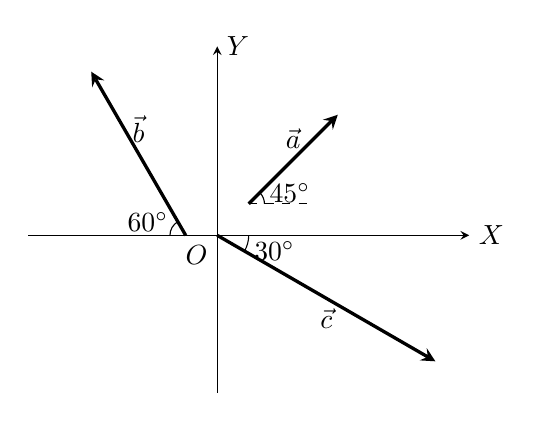
\begin{tikzpicture}[>=stealth, scale=.8]
      \draw[->](-3,0)--(4,0)node[right]{$X$};
\draw[->](0,-2.5)--(0,3)node[right]{$Y$};
\node at (0,0)[below left]{$O$};
\draw[very thick,->](.5,0.5)--node[above]{$\vec{a}$}+(45:2);
\draw[very thick,->](-.5,0)--node[above]{$\vec{b}$}+(120:3);
\draw[very thick,->](0,0)--node[below]{$\vec{c}$}(-30:4);
\draw[dashed](.5,.5)--(1.5,.5);
\draw(.75,.5) arc (0:45:.25)node[right]{$45^{\circ}$};
\draw(-.75,0) arc (180:120:.25)node[left]{$60^{\circ}$};
\draw(.5,0) arc (0:-30:.5)node[right]{$30^{\circ}$};
    \end{tikzpicture}
    \caption{}
    \end{minipage}
  \end{figure}

为了方便,在本书中我们约定,当点用大写字母标记时,它相对于原点的位置向量用相应的小写字母来标记,例
如$P$点的位置向量记为$\vec{p}$, $A$点的位置向量记为$\vec{a}$等等。

\begin{example}
    向量$\vec{a}$、$\vec{b}$、$\vec{c}$的方向与绝对值如图5.4所示,求$\vec{a}$、$\vec{b}$、$\vec{c}$的坐标。
\end{example}

\begin{solution}
设$\vec{a}=(a_x,a_y)$, $\vec{b}=(b_x,b_y)$, $\vec{c}=(c_x,c_y)$, 因此:
\[\begin{split}
a_x&=\eX\cdot \vec{a}=|\vec{a}|\cos\expval{\eX,\vec{a}}=2\cos 45^{\circ}=\sqrt{2}\\
a_y&=|\vec{a}|\cos\expval{\eY,\vec{a}}=2\cos 45^{\circ}=\sqrt{2}\\
\end{split}\]
$\therefore\quad \vec{a}=\left(\sqrt{2},\sqrt{2}\right)$
\[\begin{split}
    b_x&=|\vec{b}|\cos\expval{\eX,\vec{b}}=3\cos (180^{\circ}-60^{\circ})=-3\cos 60^{\circ}=-\frac{3}{2}\\
b_y&=|\vec{b}|\cos\expval{\eY,\vec{b}}=3\cos (90^{\circ}-60^{\circ})=3\cos30^{\circ}=\frac{3}{2}\sqrt{3}\\
\end{split}\]
$\therefore\quad \vec{b}=\left(-\frac{3}{2},\frac{3}{2}\sqrt{3}\right)$
\[\begin{split}
c_x&=|\vec{c}|\cos\expval{\eX,\vec{c}}=4\cos 30^{\circ}=2\sqrt{3}\\
c_y&=|\vec{c}|\cos\expval{\eY,\vec{c}}=4\cos (30^{\circ}+90^{\circ})=-4\sin 30^{\circ}=-2\\
\end{split}\]
$\therefore\quad \vec{c}=\left(2\sqrt{3},-2\right)$
\end{solution}

\begin{ex}
\begin{enumerate}
    \item 求图中向量的坐标。
    \item 已知$A(4, 2)$, $B(-2, 5)$, $C(-4,-3)$, $D(4,-4)$. 试用基向量$\eX,\eY$表示它们相对于原点的位置向量。
    \item 已知$\Vec{OA}=(3,-1)$, $\Vec{OB}=(2, 3)$. 试写出$A$、$B$两点的坐标。
\end{enumerate}
\end{ex}

\begin{figure}[htp]
    \centering
    \begin{minipage}[t]{0.48\textwidth}
    \centering
    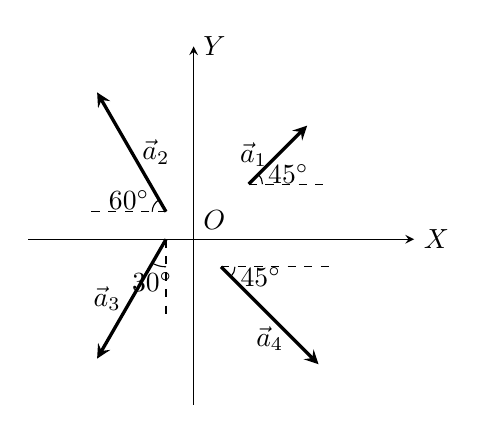
\begin{tikzpicture}[>=stealth, scale=.7]
\draw[->](-3,0)--(4,0)node[right]{$X$};
\draw[->](0,-3)--(0,3.5)node[right]{$Y$};
\node at (0,0)[above right]{$O$};
\draw[very thick,->](1,1)--node[left]{$\vec{a}_1$}+(45:1.5);
\draw[very thick,->](-.5,0.5)--node[right]{$\vec{a}_2$}+(120:2.5);
\draw[very thick,->](-.5,0)--node[left]{$\vec{a}_3$}+(-120:2.5);
\draw[very thick,->](.5,-.5)--node[below]{$\vec{a}_4$}+(-45:2.5);
\draw[dashed](1,1)--(2.5,1);
\draw[dashed](-.5,0.5)--(-2,.5);
\draw[dashed](-.5,0)--(-.5,-1.5);
\draw[dashed](.5,-.5)--(2.5,-.5);

\draw(1.25,1) arc (0:45:.25)node[right]{$45^{\circ}$};
\draw(-.75,0.5) arc (180:120:.25)node[left]{$60^{\circ}$};
\draw(-.5,-.5) arc (-90:-120:.5)node[below]{$30^{\circ}$};
\draw(.75,-.5) arc (0:-45:.25)node[right]{$45^{\circ}$};
    \end{tikzpicture}
    \caption*{第1题}
    \end{minipage}
    \begin{minipage}[t]{0.48\textwidth}
    \centering
    \begin{tikzpicture}[>=stealth, scale=.4]
\draw[->](-5,0)--(5,0)node[right]{$X$};
\draw[->](0,-5)--(0,6)node[right]{$Y$};
\node at (0,0)[below left]{$O$};
\tkzDefPoints{4/2/A, -2/5/B, -4/-3/C, 4/-4/D, 0/0/O}
\tkzDrawSegments[very thick,->](O,A O,B O,C O,D)
\tkzAutoLabelPoints[center=O](A,B,C,D)
    \end{tikzpicture}
    \caption*{第2题}
    \end{minipage}
  \end{figure}

\subsection{用向量坐标进行向量运算}
已知向量$\vec{a}=(a_x,a_y)$, $\vec{b}=(b_x,b_y)$,则
\[\vec{a}+\vec{b}= (a_x\eX+a_y\eY) +(b_x\eX+b_y\eY)= (a_x+b_x) \eX+ (a_y+b_y) \eY\]
即
\[\vec{a}+\vec{b}=(a_x,a_y)+(b_x,b_y)=(a_x+b_x,a_y+b_y) \]
同样可证:
\[\vec{a}-\vec{b}= (a_x, a_y ) -(b_x,b_y)=(a_x-b_x,a_y-b_y)\]

这就是说\textbf{向量的和与差的坐标等于各向量相应坐标的和与差}。

已知$\vec{a}=(a_x,a_y)$和一实数$\lambda$,则
\[\lambda a=\lambda (a_x\eX+a_y\eY) = \lambda a_x\eX+\lambda a_y\eY\]
即:$\lambda\vec{a}=\lambda (a_x ,a_y) = (\lambda a_x,\lambda a_y)$.

这就是说\textbf{向量倍积的坐标等于该向量相应的坐标与倍数的乘积}。

已知$\vec{a}=(a_x,a_y)$, $\vec{b}=(b_x,b_y)$, 则
\[\begin{split}
    \vec{a}\cdot \vec{b}&=(a_x\eX+a_y\eY)\cdot (b_x\eX+b_y\eY)\\
    &=a_xb_x\eX\cdot \eX+a_xb_y\eY\cdot \eX+a_yb_x\eY\eX+a_yb_y\eY\cdot \eY
\end{split}\]
由于$\eX\cdot \eX=\eY\cdot \eY=1$, $\eX\cdot \eY=\eY\cdot \eX=0$,所以
\[\vec{a}\cdot \vec{b}=(a_x,a_y)\cdot (b_x,b_y)=a_xb_x+a_yb_y\]

这就是说\textbf{两个向量内积的坐标等于两向量相应坐标的乘
积的和}。

\begin{example}
    已知$\vec{a}=(5,-3)$, $\vec{b}=(3,2)$.

求$\vec{a}+\vec{b}$, $\vec{a}-\vec{b}$, $\vec{a}\cdot \vec{b}$, $3\vec{a}+2\vec{b}$.
\end{example}

\begin{solution}
\[\begin{split}
    \vec{a}+\vec{b}&=(5,-3)+(3,2)=(8,-1)\\
    \vec{a}-\vec{b}&=(5,-3)-(3,2)=(2,-5)\\
    \vec{a}\cdot \vec{b}&=(5,-3)\cdot (3,2)=5\x 3+(-3)\x2=9\\
    3\vec{a}+2\vec{b}&=3(5,-3)+2(3,2)=(15,-9)+(6,4)=(21,-5)
\end{split}\]
\end{solution}

\begin{example}
    已知$A(x_1,y_1)$, $B(x_2,y_2)$. 求$\Vec{AB}$的坐标
(图5.5).
\end{example}

\begin{figure}[htp]
    \centering
\begin{tikzpicture}[>=stealth]
\draw[->](-2,0)--(3,0)node[right]{$X$};
\draw[->](0,-.5)--(0,3.5)node[right]{$Y$};
\node at (0,0)[below left]{$O$};
\tkzDefPoints{2/1/B, -1/3/A, 0/0/O}
\tkzDrawSegments[dashed, ->](O,A O,B)
\tkzDrawSegments[thick, ->](A,B)
\tkzLabelPoint[right](B){$B(x_2,y_2)$}
\tkzLabelPoint[left](A){$A(x_1,y_1)$}

\end{tikzpicture}
    \caption{}
\end{figure}


\begin{solution}
\[\begin{split}
    \Vec{AB}=\Vec{OB}-\Vec{OA}&=(x_2,y_2)-(x_1,y_1)\\
    &=(x_2-x_1,y_2-y_1)
\end{split}\]
\end{solution}

由例5.2我们可得到如下运算
法则:

\begin{blk}{}
    一个向量的坐标等于表示此
向量的有向线段的终点的坐标减
去起点的坐标。
\end{blk}

\begin{example}
    已知$A(3,4)$, $B(-2,7)$. 
求$\Vec{AB}$, $\Vec{BA}$; 它们的坐标之间有什么关系?
\end{example}

\begin{solution}
\[\begin{split}
    \Vec{AB}&=(-2-3,7-4)=(-5,3)\\
    \Vec{BA}&=(3-(-2),4-7)=(5,-3).
\end{split}\]
显然它们的相应的坐标分量是互为相反数。实际上
\[\Vec{BA}=(-1)\Vec{AB}=(-1)(-5,3)=(5,-3)\]
\end{solution}

\begin{example}
    已知三个向量$\vec{a}$、$\vec{b}$、$\vec{c}$,且$|\vec{a}|=|\vec{b}|=|\vec{c}|=r$. $\expval{\vec{a},\vec{b}}=\expval{\vec{b},\vec{c}}=\expval{\vec{c},\vec{a}}=120^{\circ}$
(图5.6),
求证:$\vec{a}+\vec{b}+\vec{c}=\vec{0}$.
\end{example}

\begin{figure}[htp]\centering
    \begin{minipage}[t]{0.48\textwidth}
    \centering
  \begin{tikzpicture}[>=stealth, scale=1]
    \draw[->](-2.5,0)--(2.5,0)node[right]{$X$};
    \draw[->](0,-2.5)--(0,2.5)node[right]{$Y$};
    \node at (0,0)[below right]{$O$};
    \tkzDefPoints{0/0/O, 2/0/A}
\tkzDefPoint(120:2){B}
\tkzDefPoint(-120:2){C}
\tkzDrawSegments[very thick,->](O,A O,B O,C)
\tkzLabelSegment[above](O,A){$\vec{a}$}
\tkzLabelSegment[right](O,B){$\vec{b}$}
\tkzLabelSegment[left](O,C){$\vec{c}$}
\tkzAutoLabelPoints[center=O](C,B)
\tkzLabelPoints[below](A)
    \end{tikzpicture}
    \caption{}
    \end{minipage}
    \begin{minipage}[t]{0.48\textwidth}
    \centering
    \begin{tikzpicture}[>=stealth, scale=.7]
      \draw[->](-3,0)--(5,0)node[right]{$X$};
\draw[->](0,-1)--(0,6)node[right]{$Y$};
\node at (0,0)[below left]{$O$};
\tkzDefPoints{0/1/A, 4/3/B, 2/5/C, 0/0/O}
\tkzDefPointsBy[translation = from B to C](A){D}
\tkzDrawPolygon[very thick](A,B,C,D)
\tkzDrawSegments[dashed, ->](O,D O,A)
\tkzLabelPoints[above](B,C,D)
\tkzLabelPoints[below right](A)
    \end{tikzpicture}
    \caption{}
    \end{minipage}
    \end{figure}

\begin{proof}
    设$\Vec{OA}=\vec{a}$, $\Vec{OB}=\vec{b}$, 
$\Vec{OC}=\vec{c}$, 以$\Vec{OA}$的方向作为$X$轴
的正方向建立坐标系$[O:\; \eX,\eY]$
则 
\[\begin{split}
    \Vec{OA}&=(r, 0)\\
    \Vec{OB}&=\left(|\vec{b}|\cos120^{\circ}, |\vec{b}|\cos 30^{\circ}\right)=\left(-\frac{r}{2},\frac{\sqrt{3}}{2}r\right)\\
    \Vec{OC}&=\left(|\vec{c}|\cos120^{\circ}, |\vec{c}|\cos 150^{\circ}\right)=\left(-\frac{r}{2},-\frac{\sqrt{3}}{2}r\right)\\
    \Vec{OA}+  \Vec{OB}+\Vec{OC}&=(r,0)+\left(-\frac{r}{2},\frac{\sqrt{3}}{2}r\right)+\left(-\frac{r}{2},-\frac{\sqrt{3}}{2}r\right)\\
    &=\left(r-\frac{r}{2}-\frac{r}{2}, 0+\frac{\sqrt{3}}{2}-\frac{\sqrt{3}}{2}\right)=(0,0)
\end{split}\]
$\therefore\quad \vec{a}+\vec{b}+\vec{c}=\vec{0}$.
\end{proof}

\begin{example}
    已知$\parallelogram{ABCD}$, $A(0,1)$、$B(4,3)$、
$C(2,5)$

求顶点$D$的坐标(图5.7).
\end{example}

\begin{solution}
\[\begin{split}
\Vec{OD}=\Vec{OA}+\Vec{AD}&=\Vec{OA}+\Vec{BC}\\
&=\Vec{OA}+\Vec{OC}-\Vec{OB}\\
&=(0,1)+(2,5)-(4,3)=(-2,3)
\end{split}\]
所以$D$的坐标是$(-2,3)$.
\end{solution}

\begin{ex}
\begin{enumerate}
    \item 已知$\vec{a}=(-5,3)$, $\vec{b}=(7,-2)$. 求$\vec{a}+\vec{b}$, $\vec{a}-\vec{b}$, $\vec{a}\cdot \vec{b}$, $4\vec{a}-7\vec{b}$的坐标。

    \item 已知$\vec{a}=(2,-1)$, $\vec{b}=(-1,1)$. 求$\vec{a}+\vec{b}$, 
    $\vec{a}-\vec{b}$的坐标,并画图验证。
    \item 已知$\vec{a}=(1,2)$, $\vec{b}=(3,1)$. 试以$O$为起点画有
    向线段,分别表示$\vec{a}+\vec{b}$, $\vec{a}-\vec{b}$, $2\vec{a}-3\vec{b}$.
    \item 已知$\vec{a}=(1,2)$, $\vec{b}=(-2,3)$. 求
\begin{multicols}{2}
\begin{enumerate}
    \item $\vec{a}\cdot \vec{b}$, 
    \item $(\vec{a}+\vec{b})\cdot (\vec{a}+\vec{b})$, 
    \item $(\vec{a}+\vec{b})\cdot (\vec{a}-\vec{b})$, 
    \item $(\vec{a}-\vec{b})\cdot (\vec{a}-\vec{b})$.
\end{enumerate}
\end{multicols}
    
\item 已知$\vec{a}=(\sqrt{2},-1)$, $\vec{b}=(-\sqrt{3},3)$. 求
\begin{multicols}{3}
  \begin{enumerate}
      \item $\vec{a}\cdot \vec{b}$
      \item $(4\vec{a}-\vec{b})\cdot (4\vec{a}+\vec{b})$
      \item $(\vec{a}-2\vec{b})\cdot (\vec{a}-2\vec{b})$
  \end{enumerate}  
\end{multicols}

\item 已知$\parallelogram{ABCD}$的三个顶点$A(0,0)$, $B(3,1)$, 
$C(4,3)$. 试求顶点$D$的坐标。
\item 已知$O$是正六边形$ABCDEF$的中心,用向量坐标运算证明:
\[\Vec{OA}+\Vec{OB}+\Vec{OC}+\Vec{OD}+\Vec{OE}+\Vec{OF}=\vec{0}\]
   \end{enumerate} 
\end{ex}

\subsection{垂直与平行向量的坐标关系}

已知$\vec{a}$、$\vec{b}\; (\vec{b}\ne \vec{0})$平行的充要条件是存在一个实数
$\lambda$使等式
\[\vec{a}=\lambda\vec{b}\]
成立。如果$\vec{a}=(a_x,a_y)$, $\vec{b}=(b_x,b_y)$, 
那么上面的充
要条件用坐标表示,可写为:
\[(a_x,a_y)=(\lambda b_x,\lambda b_y)\]
即:
\[\begin{cases}
    a_x=\lambda b_x\\
a_y=\lambda b_y
\end{cases}\]

由上式消去$\lambda$, 上述条件又可写为:
\[\begin{vmatrix}
    a_x& a_y\\b_x&b_y
\end{vmatrix}=0\]
或:$a_x:b_x=a_y:b_y$.

上述结论可叙述为如下定理。

\begin{blk}
    {定理} 两个向量平行的一个充分必要条件是它们相应的
坐标分量成比例。
\end{blk}

\begin{blk}
{推论} 如果$A(x_1,y_1)$, $B(x_2,y_2)$, $C(x_3,y_3)$
是坐标平面上三个不同的点,那么$A$、$B$、$C$三点共线的-
个充要条件是
\[\frac{x_2-x_1}{x_3-x_1}=\frac{y_2-y_1}{y_3-y_1}\]
或者用三阶行列式写为
\[\begin{vmatrix}
    x_1&y_1&1\\
    x_2&y_2&1\\
    x_3&y_3&1\\
\end{vmatrix}=0\]
\end{blk}

\begin{proof}
    因为
\[\Vec{AB}=(x_2-x_1,y_2-y_1),\qquad \Vec{AC}=(x_3-x_1,y_3-y_1)\]
由于$A$、$B$、$C$三点共线的充要条件是
$\Vec{AB}\parallel \Vec{AC}$,所以,由上述定理便得到
\[\frac{x_2-x_1}{x_3-x_1}=\frac{y_2-y_1}{y_3-y_1}\]
即:$\begin{vmatrix}
    x_1&y_1&1\\
    x_2&y_2&1\\
    x_3&y_3&1\\
\end{vmatrix}=0$
从行列式计算法则容易证明:
\[\begin{vmatrix}
    x_2-x_1&x_3-x_1\\
    y_2-y_1&y_3-y_1
\end{vmatrix}=\begin{vmatrix}
    x_1&y_1&1\\
    x_2&y_2&1\\
    x_3&y_3&1\\
\end{vmatrix}=0\]
\end{proof}

我们已知
\[\vec{a}\bot\vec{b}\quad \Longleftrightarrow \quad \vec{a}\cdot \vec{b}=0\]
如果$\vec{a}=(a_x,a_y)$、$\vec{b}=(b_x,b_y)$, 那么上述条件用坐标
表示可写为
\[\vec{a}\bot\vec{b}\quad \Longleftrightarrow \quad a_xb_x+a_yb_y=0\]

这也可写为如下定理:

\begin{blk}
  {定理} 两个向量垂直的充要条件是它们相应坐标的乘积
的和等于零。  
\end{blk}

\begin{example}
    已知$\vec{a}=(3,y)$, $\vec{b}=(6,4)$且$\vec{a}\parallel \vec{b}$. 求$y$值。
\end{example}

\begin{solution}
    因为$\vec{a}\parallel \vec{b}$,所以
    \[\frac{6}{3}=\frac{4}{y}\]
    解之得$y=2$. 
\end{solution}

\begin{example}
已知$A(1,1)$, $B(3,5)$, $C(-2,-5)$.
问:$A$、$B$、$C$三点是否共线。
\end{example}

\begin{solution}
因为$\Vec{AB}=(2,4)$, $\Vec{AC}=(-3,-6)$,
且
\[\begin{vmatrix}
    2&4\\
    -3&-6
\end{vmatrix}=-12+12=0\]
所以$A$、$B$、$C$三点共线。
\end{solution}
    
\begin{example}
    已知$\vec{a}=(3,2)$, $\vec{b}=(-6,9)$. 求证$\vec{a}\bot\vec{b}$.
\end{example}

\begin{solution}
因为
\[\vec{a}\cdot \vec{b}=3\x (-6)+2\x 9=-18+18=0\]
所以$\vec{a}\bot\vec{b}$.
\end{solution}

\begin{example}
    已知$A(1,2)$, $B(2,3)$, $C(-2,5)$。
    求证$\triangle ABC$是直角三角形。
\end{example}


\begin{solution}
因为
\[\begin{split}
    \Vec{AB}&=(2,3)-(1,2)=(1,1)\\
    \Vec{AC}&=(-2,5)-(1,2)=(-3,3)\\
    \Vec{AB}\cdot \Vec{AC}&=1\x(-3)+1\x3=0
\end{split}\]
    所以$\Vec{AB}\bot \Vec{AC}$, 即$\triangle ABC$是直角三角形。
\end{solution}

\begin{ex}
\begin{enumerate}
    \item 试问下列向量是否平行。
    \begin{enumerate}
    \item $\vec{a}=\left(\frac{1}{2},\frac{3}{4}\right),\quad \vec{b}=(-2,-3)$
    \item $\vec{p}=(0.5,4),\quad \vec{q}=(-8,64)$
    \item $\vec{c}=(2,3),\quad \vec{d}=(3,4)$
\end{enumerate}

\item 已知$\vec{a}=\left(\frac{3}{5},-5\right)$, $\vec{b}=(3,y)$, 且$\vec{a}\parallel \vec{b}$, 求$y$.

\item 向量$\vec{a}=(5,7)$与$\vec{b}=(10,14)$是否共线。

\item 已知$\vec{a}=(1,3)$, $\vec{b}=(2,5)$, 求证$\vec{a},\vec{b}$线性无
关。

\item 已知$\vec{a}=(-3,2)$, $\vec{b}=(4,6)$. 求证$\vec{a}\bot \vec{b}$, 并
作图验证。

\item 已知$A(7,5)$, $B(2,3)$, $C(6,-7)$. 求证
$\triangle ABC$是直角三角形。
\end{enumerate}
\end{ex}

\subsection{有向线段定比分点的坐标}
已知点$P$按定比$\mu$分割有向线段$P_1P_2$(图5.8). 
即
\[\begin{split}
     \Vec{P_1P}&=\mu \Vec{PP_2}\\
     \Vec{OP}-\Vec{OP_1}&=\mu\left(\Vec{OP_2}-\Vec{OP}\right)
\end{split}\]
所以
\[\Vec{OP}=\frac{1}{1+\mu}\Vec{OP_1}+\frac{\mu}{1+\mu}\Vec{OP_2}\]

\begin{figure}[htp]
    \centering
\begin{tikzpicture}[>=stealth]
\draw[->](-1,0)--(4,0)node[right]{$X$};
\draw[->](0,-1)--(0,3.5)node[right]{$Y$};
\node at (0,0)[below left]{$O$};
\tkzDefPoints{-1/3/A, 3/-1/B, 0/0/O, -.5/2.5/P, 1/1/P_2, 2.5/-.5/P_1}
\tkzDrawSegments[thick](A,B)
\tkzDrawSegments[->, very thick](O,P O,P_1 O,P_2)
\tkzLabelPoints[right](P,P_1,P_2)

\end{tikzpicture}
    \caption{}
\end{figure}


如果$\Vec{OP_1}=(x_1,y_1)$,$\Vec{OP_2}=(x_2,y_2)$, $\Vec{OP}=(x,y)$,那么上式用坐标表示即可写为
\[(x,y)=\left(\frac{x_1+\mu x_2}{1+\mu},\; \frac{y_1+\mu y_2}{1+\mu}\right)\]
即:
\[x=\frac{x_1+\mu x_2}{1+\mu},\qquad y=\frac{y_1+\mu y_2}{1+\mu}\]
这就是求有向线段定比分点的计算公式。

当$\mu=1$时,$P$点是线段$\overline{P_1P_2}$的中点。这时$P$点的坐
标是
\[x=\frac{x_1+ x_2}{2},\qquad y=\frac{y_1+y_2}{2}\]
这就是求线段中点的坐标的计算公式,通常叫做\textbf{中点公式}。

\begin{figure}[htp]\centering
    \begin{minipage}[t]{0.48\textwidth}
    \centering
  \begin{tikzpicture}[>=stealth, scale=.5]
    \draw[->](-1,0)--(7,0)node[right]{$X$};
    \draw[->](0,-3)--(0,7)node[right]{$Y$};
    \node at (0,0)[below left]{$O$};
\tkzDefPoints{1/3/A, 4/-2/B, 2/1.333/P}
\tkzDrawLines[very thick, add = .6 and .2](A,B)
\tkzDrawPoints(A,B,P)
\tkzLabelPoints[right](A,B)
\tkzLabelPoint[right](P){$P(2,\tfrac{4}{3})$}
\foreach \x in {1,2,3,4}
{
    \draw(\x,0)--(\x,.2);
    \draw(0,\x)--(.2,\x);
}
    \end{tikzpicture}
    \caption{}
    \end{minipage}
    \begin{minipage}[t]{0.48\textwidth}
    \centering
    \begin{tikzpicture}[>=stealth, scale=1]
    \draw[->](-.5,0)--(4,0)node[right]{$X$};
    \draw[->](0,-.5)--(0,4)node[right]{$Y$};
    \node at (0,0)[below left]{$O$};
\tkzDefPoints{1/1/A, 2/2/B, 3/3/P}
\draw[very thick](0,0)--(3.5,3.5);
\tkzDrawPoints(A,B,P)
\tkzLabelPoints[left](A,B)
\tkzLabelPoint[right](P){$P(3,3)$}
    \end{tikzpicture}
    \caption{}
    \end{minipage}
    \end{figure}


\begin{example}
    已知$A(1,3)$, $B(4,-2)$. 点$P$按定比$\frac{1}{2}$
分割$\Vec{AB}$, 求$P$点的坐标(图5.9).
\end{example}

\begin{solution}
因$\mu=\frac{1}{2}$, 由求定比分点坐标计算公式得:
\[
    x=\frac{1+\frac{1}{2}\x 4}{1+\frac{1}{2}}=2,\qquad
    y=\frac{3+\frac{1}{2}\x (-2)}{1+\frac{1}{2}}=\frac{4}{3}
\]
所以$P\left(2,\frac{4}{3}\right)$.
\end{solution}

\begin{example}
    已知$A(1,1)$, $B(2,2)$, 点$P$按定比$-\frac{1}{2}$
分割$\Vec{BA}$, 求$P$点的坐标(图5.10).
\end{example}

\begin{solution}
因$\mu=-\frac{1}{2}$, 由求定比分点坐标计算公式得:
\[
    x=\frac{2+\left(-\frac{1}{2}\right)\x 1}{1+\left(-\frac{1}{2}\right)}=3,\qquad
    y=\frac{2+\left(-\frac{1}{2}\right)\x 1}{1+\left(-\frac{1}{2}\right)}=3
\]
所以$P(3,3)$.
\end{solution}

在使用定比分点公式时,请同学们注意有向线段的起点
和终点,以避免出错。

\begin{ex}
\begin{enumerate}
    \item 已知:
\begin{enumerate}
    \item $A(3,5),\quad B(-3,7)$
    \item $A(4,-1),\quad B(-5,-6)$
    \item $A(a+b,c+d),\quad B(a-b,c-d)$
\end{enumerate}
    试求$\Vec{AB}$的中点的坐标。
    \item 已知$P(0,2)$, $Q(2,-1)$, 点$M$按定比$\frac{1}{2}$分割
    $\Vec{PQ}$, 点$N$按定比3分割$\Vec{QP}$, 求$M$、$N$两点的坐标。
    \item 已知$M_1(-1,6)$, $M_2(4,3)$, 求$\Vec{M_1M_2}$三等分点
    的坐标。
    \item 已知$A_1(x_1,y_1)$, $A_2(x_2,y_2)$, $A_3(x_3,y_3)$是$\triangle A_1A_2A_3$的三个顶点,求$\triangle A_1A_2A_3$的重心的坐
    标。
    \item 已知$A(1,2)$, $B(3,4)$, 
    $|\Vec{AP}|=2|\Vec{AB}|$,求$P$点的坐标。
    \item 已知点$B(-4,1)$到点$A(2,-2)$的距离是它到点
    $C(x,y)$的距离的一半,求$C(x,y)$.
    \item 已知$\parallelogram{ABCD}$的相邻两顶点$A(1,1)$, $B(3,2)$
    和它的对角线交点$K(2,3)$, 求其余两个顶点的坐
    标。
\end{enumerate}
\end{ex}

\subsection{向量的长度公式}
如果已知$\vec{a}=(a_x,a_y)$, 则
\[|\vec{a}|^2=\vec{a}\cdot \vec{a}=a_x^2+a^2_y\]
所以
\begin{equation}
    |\vec{a}|=\sqrt{a_x^2+a^2_y}
\end{equation}
(5.4)式就是求$\vec{a}$的\textbf{长度的计算公式}。

如果已知两点$A(x_1,y_1)$, $B(x_2,y_2)$ (图5.11),
则
\[\Vec{AB}=(x_2-x_1,y_2-y_1)\]

\begin{figure}[htp]
    \centering
\begin{tikzpicture}[>=stealth]
    \draw[->](-.5,0)--(4,0)node[right]{$X$};
    \draw[->](0,-.5)--(0,4)node[right]{$Y$};
    \node at (0,0)[below left]{$O$};
\tkzDefPoints{2/1/A, 3/3/B}
\tkzDrawSegments[very thick,->](A,B)
\draw[dashed](0,1)--(A)--(2,0);
\draw[dashed](0,3)--(B)--node[right]{$a_y$}(3,1)--(3,0);
\draw[dashed](A)--node[below]{$a_x$}(3,1);
\tkzLabelSegment[left](A,B){$\vec{a}$}
\tkzLabelPoints[above](B)
\tkzLabelPoints[below left](A)

\end{tikzpicture}
    \caption{}
\end{figure}


\begin{equation}
    |\Vec{AB}|=\sqrt{(x_2-x_1)^2+(y_2-y_1)^2}
\end{equation}
显然$A$、$B$两点间的距离就是
$|\Vec{AB}|$,所以(5.5)式是求两
点间的\textbf{距离公式}。它可叙述如下:

\textbf{两点间的距离等于两点相应坐标差的平方和的算术平方
根}。

如果$\vec{a}_0$是$\vec{a}$的单位向量,$\vec{a}=(a_x,a_y)$, 
那么,
\[\vec{a}_0=\frac{1}{|\vec{a}|}\vec{a}=\frac{1}{\sqrt{a^2_x+a^2_y}}(a_x,a_y)\]
即
\begin{equation}
    \vec{a}_0=\left(\frac{a_x}{\sqrt{a^2_x+a^2_y}},\; \frac{a_y}{\sqrt{a^2_x+a^2_y}}\right)
\end{equation}
它是由已知向量的坐标,求它的单位向量的坐标的计算公
式。

\begin{example}
    已知$A(3,6)$, $B(-2,3)$. 求$A$、$B$间距
离。
\end{example}

\begin{solution}
    因$\Vec{AB}=(-5,-3)$, 所以
\[|\Vec{AB}|=\sqrt{(-5)^2+(-3)^2}=\sqrt{34}\]
\end{solution}


\begin{example}
    已知$\vec{a}=(3,4)$, 求$\vec{a}_0$的坐标。
\end{example}

\begin{solution}
因为$|\vec{a}|=\sqrt{3^2+4^2}=5$, 所以
\[\vec{a}_0=\left(\frac{3}{5},\frac{4}{5}\right)\]
\end{solution}

\begin{example}
    已知$A(1,2)$, $B(3,4)$, $C(5,0)$. 求证:$\triangle ABC$是等腰三角形。
\end{example}

\begin{proof}
\[\begin{split}
|\Vec{AB}|&=\sqrt{(3-1)^2+(4-2)^2}=\sqrt{8}\\
|\Vec{AC}|&=\sqrt{(5-1)^2+(0-2)^2}=\sqrt{20}\\
|\Vec{BC}|&=\sqrt{(5-3)^2+(0-4)^2}=\sqrt{20}\\
\end{split}\]
由此得$|\Vec{AC}|=|\Vec{BC}$, 所以$\triangle ABC$是等腰三角形。
\end{proof}

\begin{ex}
\begin{enumerate}
    \item 已知$A(0,0)$, $B(3,4)$, $C(0,5)$, 求$\triangle ABC$
    各边的长。
    \item 已知$A(3,8)$, $B(-11,3)$, $C(-8,-2)$. 求
    证$\triangle ABC$是等腰三角形。
    \item 已知$A(-1,2)$, $B(3,5)$, $C(1,7)$, 
    $D(-3,4)$, 求证$ABCD$是平行四边形,且求其对
    角线的长度。
    \item 已知$\vec{a}=(1,1)$, $\vec{b}=(-2,5)$, 求$\vec{a}_0$, $\vec{b}_0$.
    \item 已知$|\vec{a}|=5$, 且$\vec{a}_0=\left(\frac{2}{\sqrt{13}},\frac{3}{\sqrt{13}}\right)$,
    求$\vec{a}$的坐标。
    \item 用坐标法证明:如果$M$是$\triangle ABC$的$\overline{BC}$
    边上的中点,
    求证:$\overline{AB}^2+\overline{AС}^2=2\overline{AМ}^2+2\overline{BM}^2$.
\end{enumerate}
\end{ex}

\subsection{两向量的夹角计算公式}

已知$\vec{a}=(a_x,a_y)$, $\vec{b}=(b_x,b_y)$, 则
\[\cos\expval{\vec{a},\vec{b}}=\frac{\vec{a}\cdot \vec{b}}{|\vec{a}|\left|\vec{b}\right|}\]
但$\vec{a}\cdot \vec{b}=a_xb_x+a_yb_y,\quad |\vec{a}|=\sqrt{a_x^2+a_y^2},\quad \left|\vec{b}\right|=\sqrt{b_x^2+b_y^2}$,
所以
\begin{equation}
    \cos\expval{\vec{a},\vec{b}}=\frac{a_xb_x+a_yb_y}{\sqrt{a_x^2+a_y^2}\sqrt{b_x^2+b_y^2}}
\end{equation}
(5.7)式是求两个向量夹角的\textbf{余弦的计算公式}。由两个向量
夹角的余弦,我们就可求出这两个向量的夹角。

设$\expval{\eX,\vec{a}}=\alpha$, $\expval{\eY,\vec{a}}=\beta$,已知
\[a_x=|\vec{a}|\cos\alpha,\qquad a_y=|\vec{a}|\cos\beta\]
则
\begin{equation}
    \begin{cases}
\cos\alpha=\frac{a_x}{|\vec{a}|}=\frac{a_x}{\sqrt{a_x^2+a_y^2}}\\
\cos\beta=\frac{a_y}{|\vec{a}|}=\frac{a_y}{\sqrt{a_x^2+a_y^2}}\\
    \end{cases}
\end{equation}
但由(5.6)式知
\[\vec{a}_0=\left(\frac{a_x}{\sqrt{a_x^2+a_y^2}},\; \frac{a_y}{\sqrt{a_x^2+a_y^2}}\right)\]
所以:$\vec{a}_0=(\cos\alpha,\cos\beta)$. 这就是说$(\cos\alpha,\cos\beta)$就是$\vec{a}$的单位向量的坐标。

容易验证$\cos\alpha,\; \cos\beta$之间满足关系
\begin{equation}
    \cos^2\alpha+\cos^2\beta=1
\end{equation}
(5.8)、(5.9)是两个重要的公式,它们把向量的坐标与向
量的长度、方向联系起来。

\begin{example}
  已知$A(\sqrt{3},1)$, $B(0,1)$, 
$c\left(\frac{\sqrt{3}}{2},\frac{1}{2}\right)$, 
求$\Vec{AB}$与$\Vec{AC}$之间的夹角。  
\end{example}

\begin{solution}
因为$\Vec{AB}=(-\sqrt{3},0)$, $\Vec{AC}=\left(-\frac{\sqrt{3}}{2},\frac{1}{2}\right)$, 所以
\[\cos \expval{\Vec{AB},\Vec{AC}} =\frac{-\sqrt{3}\x\left(-\frac{\sqrt{3}}{2}\right)+0\x \left(-\frac{1}{2}\right)}{\sqrt{\left(\sqrt{3}\right)^2+0^2}\sqrt{\left(-\frac{\sqrt{3}}{2}\right)^2+\left(-\frac{1}{2}\right)^2}}=\frac{\sqrt{3}}{2}\]
因此,
\[\expval{\Vec{AB},\Vec{AC}}=\frac{\pi}{6}\]
\end{solution}

\begin{example}
    求向量$\vec{a}=(2,-1)$的方向余弦和$\vec{a}_0$的坐标。
\end{example}

\begin{solution}
因为$|\vec{a}|=\sqrt{2^2+(-1)^2}=\sqrt{5}$,所以
\[\cos\alpha=\frac{2}{\sqrt{5}},\qquad \cos\beta=\frac{-1}{\sqrt{5}}\]
\[\vec{a}_0=(\cos\alpha,\cos\beta)=\left(\frac{2}{\sqrt{5}},-\frac{1}{\sqrt{5}}\right)\]
\end{solution}

\begin{ex}
\begin{enumerate}
    \item 求下列$\vec{a}$与$\vec{b}$夹角的余弦。
\begin{enumerate}
    \item $\vec{a}=(1,-2),\quad \vec{b}=(5,3)$
    \item $\vec{a}=(-3,4),\quad \vec{b}=(2,-1)$
\end{enumerate}  
    \item 求下列向量的单位向量的坐标。
\begin{multicols}{2}
\begin{enumerate}
    \item $\vec{a}=(2,3)$
    \item $\vec{b}=(5,13)$
    \item $\vec{c}=(2,0)$
    \item $\vec{d}=(1,1)$
\end{enumerate}
\end{multicols}
    \item 已知$\Vec{OA}=(-1,3)$, 
    $\Vec{OB}=(0,4)$, 求$\Vec{OA}$在
    $\Vec{OB}$上的垂直投影分量,$\Vec{OB}$在$\Vec{OA}$上的垂直投影分
    量。
    \item 已知$A(2,-1)$, $B(1,-3)$, $C(3,-4)$, 计
    算$\triangle ABC$的三内角的余弦。
\end{enumerate} 
\end{ex}

\subsection{两向量方向差的正弦、正切公式}
由于我们规定两个向量的夹角取值范围是$[0,\pi]$,
所以在坐标平面上知道$\expval{\eX,\vec{a}}$和$\expval{\eY,\vec{a}}$这两个角$\vec{a}$
的方向唯一确定了,其实在坐标平面上只需要知道其中一个
角就够了。

在坐标系$[O:\; \eX,\eY]$中(图5.12),已知非零向
量$\vec{a}=(a_x,a_y)$, 作$\Vec{OA}=\vec{a}$, 
这时射线$OA$的方向被以$OX$为
始边、$OA$为终边的旋转角$\varphi$所
唯一确定,于是$\vec{a}$的方向也被$\varphi$
所唯一确定。$\varphi$角通常叫做向量
$\vec{a}$的\textbf{方向角}。由三角学可知,$\varphi$
有无穷多值,因此平面上同一个
方向可以和无穷多个角相对应。如果约定$\varphi$在$[0,2\pi]$内
取值,一个向量的方向角就被唯一确定了。

\begin{figure}[htp]
    \centering
    \begin{tikzpicture}[>=stealth]
    \draw[->](-.5,0)--(4,0)node[right]{$X$};
    \draw[->](0,-.5)--(0,3.5)node[right]{$Y$};
    \node at (0,0)[below left]{$O$};
    \tkzDefPoints{0/0/O, 3/2.5/A, 2/0/B}
    \tkzDrawSegments[very thick, ->](O,A)
    \tkzLabelPoints[above](A)
    \tkzLabelSegment[above](O,A){$\vec{a}$}
\tkzMarkAngles[mark=none,size=1,->](B,O,A)
\tkzLabelAngle[pos=1.3](B,O,A){$\varphi$}        
    \end{tikzpicture}
    \caption{}
\end{figure}

我们曾规定$\expval{\eX,\vec{a}}=\alpha$, $\expval{\eY,\vec{a}}=\beta$的取值范
围是$[0,\pi]$. 因此上述定义的角$\varphi$和角$\alpha$并不一致。但
我们知道
\[\cos\alpha=\frac{a_x}{|\vec{a}|},\qquad \cos\beta=\frac{a_y}{|\vec{a}|}\]
由三角函数的定义,我们又知
\[\cos\varphi=\frac{a_x}{|\vec{a}|},\qquad \sin\varphi=\frac{a_y}{|\vec{a}|}\]
所以不论$\varphi$取何值,都有关系式
\[\cos\varphi=\cos\alpha,\qquad \sin\varphi=\cos\beta\]
因此一个向量的方向余弦,用它的方向角可表示为$\cos\varphi$, $
\sin\varphi$. 任给一单位向量$\vec{e}$, 若方向角为$\varphi$, 则
\[\vec{e}=(\cos\varphi,\; \sin\varphi)\]

在(5.10)式两边相除可得
\[\tan \varphi =\frac{a_y}{a_x}\]

\begin{figure}[htp]
    \centering
\begin{tikzpicture}[>=stealth]
\draw[->](-3,0)--(3,0)node[right]{$X$};
\draw[->](0,-.5)--(0,3.5)node[right]{$Y$};
\tkzDefPoints{2.5/2/A, -2.5/2.5/B, 3/0/C, 0/0/O}
\tkzDrawSegments[very thick, ->](O,A O,B)
\tkzLabelSegment[below](O,B){$\vec{b}$}
\tkzLabelSegment[above](O,A){$\vec{a}$}
\tkzLabelPoints[above](A,B)
\tkzLabelPoints[below left](O)
\tkzMarkAngles[size=1, mark=none, ->](C,O,A)
\tkzMarkAngles[size=.8, mark=none, ->](C,O,B)
\tkzMarkAngles[size=1.5, mark=none, ->](A,O,B)
\tkzLabelAngle[pos=1.3](C,O,A){$\varphi_1$}
\tkzLabelAngle[pos=1.1](C,O,B){$\varphi_2$}
\tkzLabelAngle[pos=1.8](A,O,B){$\varphi$}

\end{tikzpicture}
    \caption{}
\end{figure}


已知$\vec{a}=(a_x,a_y)$, $\vec{b}=(b_x,b_y)$, 作$\Vec{OA}=\vec{a}$, $\Vec{OB}=\vec{b}$ (图5.13), 设$\vec{a}$的方向角为$\varphi_1$, $\vec{b}$的方向角
为$\varphi_2$, 我们把$\vec{b}$与$\vec{a}$的方向差$\varphi$定义为
$\varphi=\varphi_2-\varphi_1$,
这就是说$\varphi$是射线$OA$到射线
$OB$之间的旋转角,也可说$\varphi$ 
是$\vec{a}$到$\vec{b}$的旋转角。容易证
明,对任意两个向量$\vec{a},\vec{b}$, 
有
\[\cos\varphi =\cos\expval{\vec{a},\vec{b}}\]
由三角公式有
\[\sin\varphi  =\sin(\varphi_2-\varphi_1 ) = \sin\varphi_2\cos\varphi_1 -\cos\varphi_2\sin\varphi_1\]
但
\[\sin\varphi_2=\frac{b_y}{|\vec{b}|},\quad \cos\varphi_2=\frac{b_x}{|\vec{b}|},\quad \sin\varphi_1=\frac{a_y}{|\vec{a}|},\quad \cos\varphi_1=\frac{a_x}{|\vec{a}|}\]
所以
\begin{equation}
    \sin\varphi=\frac{a_xb_y-a_yb_x}{|\vec{a}|\left|\vec{b}\right|}
\end{equation}
又知
\[\cos\varphi =\cos\expval{\vec{a},\vec{b}}=\frac{a_xb_x+a_yb_y}{|\vec{a}|\left|\vec{b}\right|}\]
两式相除又可得
\[\tan\varphi =\frac{a_xb_y-a_yb_x}{a_xb_x+a_yb_y}\]
为了便于记忆,(5.10)、(5.11)两式还可用行列式写出:
\[\sin\varphi=\frac{\begin{vmatrix}
    a_x& a_y\\b_x&b_y
\end{vmatrix}}{|\vec{a}|\left|\vec{b}\right|},\qquad \tan\varphi=\frac{\begin{vmatrix}
    a_x& a_y\\b_x&b_y
\end{vmatrix}}{\vec{a}\cdot \vec{b}}\]


\begin{example}
    已知$\vec{a}=(2,-2)$, 求$\vec{a}$的方向角$\varphi$.
\end{example}

\begin{solution}
    因为$\sin\varphi=\frac{-2}{\sqrt{2^2+(-2)^2}}=-\frac{1}{\sqrt{2}}$,所以,$\varphi=-45^{\circ}$或$\varphi=-135^{\circ}$, 又因$\cos\varphi$的值为正($\cos\varphi$与$\vec{a}$的
横坐标同号),所以$\varphi=-45^{\circ}$.
\end{solution}


\begin{example}
    已知$\vec{a}=(\sqrt{3},0)$, $\vec{b}=\left(\frac{\sqrt{3}}{2},-\frac{1}{2}\right)$, 求$\vec{a}$与$\vec{b}$的方向差$\varphi$.
\end{example}

\begin{solution}
因为$|\vec{a}|=\sqrt{3}$, $|\vec{b}|=\sqrt{\left(\frac{\sqrt{3}}{2}\right)^2+\left(-\frac{1}{2}\right)^2}=1$
所以
\[\cos\varphi=\frac{a_xb_x+a_yb_y}{|\vec{a}|\left|\vec{b}\right|}=\frac{\sqrt{3}\cdot \frac{\sqrt{3}}{2}+0\cdot \left(-\frac{1}{2}\right)}{\sqrt{3}\cdot 1}=\frac{\sqrt{3}}{2}\]
于是$\varphi=\frac{\pi}{6}$, 或$\varphi=-\frac{11}{6}\pi$. 又因为
\[\sin\varphi=\frac{a_xb_y-a_yb_x}{|\vec{a}|\left|\vec{b}\right|}=\frac{\sqrt{3}\x \left(-\frac{1}{2}\right)+0\x \frac{\sqrt{3}}{2}}{\sqrt{3}\cdot 1}=-\frac{1}{2}\]
所以:$\varphi=-\frac{11}{6}\pi$.
\end{solution}

由例5.19可知,如果我们要求两向量的夹角,只用余弦公
式就可以了,如果要计算两向量的方向差,除用余弦公式
外,还要用正弦公式或正切公式。


\begin{example}
    已知$\vec{a}=(a_x,a_y)$, 求与$\vec{a}$垂直的单位向量$\vec{n}_0$的坐标。
\end{example}

\begin{solution}
    设$\vec{n}_0=(\cos\varphi,\sin\varphi)$,由于$\vec{n}_0\bot \vec{a}$, 所以
\[a_x\cos\alpha+a_y\sin\alpha= 0\]
即:$\frac{\cos\alpha}{-a_y}=\frac{\sin\alpha}{a_x}$.

由此可见,向量$\vec{n}_0$与向量$(-a_y,a_x)$平行。
于是存在数$\lambda$, 使
\[\cos\varphi=\lambda(-a_y),\qquad \sin\varphi=\lambda a_x\]
由于$\sin^2\varphi +\cos^2\varphi =1$, 因此可求得
\[\lambda=\pm\frac{1}{\sqrt{a^2_x+a^2_y}}=\pm\frac{1}{|\vec{a}|}\]
所以
\[\begin{split}
    \cos\varphi&=\pm\frac{1}{|\vec{a}|}\x (-a_y)=\mp\frac{a_y}{|\vec{a}|}\\
    \sin\varphi&=\pm\frac{a_x}{|\vec{a}|}
\end{split}\]
于是可得:
\[\vec{n}_0=\left(-\frac{a_y}{|\vec{a}|},\; \frac{a_x}{|\vec{a}|}\right)\quad \text{或}\quad \vec{n}_0=\left(\frac{a_y}{|\vec{a}|},\; -\frac{a_x}{|\vec{a}|}\right)\]
\end{solution}

求一个向量的垂直向量的坐标,是我们经常要碰到的问
题,我们在例5.20的基础上,再作些说明:

由于$\vec{n}_0\bot \vec{a}$, 因此对任意实数$k$
\[k\vec{n}_0\bot \vec{a}\]
特别当$k=\pm|\vec{a}|$时,向量$\vec{n}_1=(-a_y,a_x)$, $\vec{n}_2=(a_y,-a_x)$
都与$\vec{a}$垂直,且与$\vec{a}$的长度相等。例如$\vec{a}=(3,4)$, 则$\vec{n}_1=(-4,3)$, $\vec{n}_2=(4,-3)$
都垂直于$\vec{a}$ (图5.14).

令$\varphi_1$是$\vec{n}_1$与$\vec{a}$的方向差,$\varphi_2$是$\vec{n}_2$与$\vec{a}$的方向差,则
\[\begin{split}
\sin\varphi_1&=\frac{\begin{vmatrix}
    a_x&a_y\\-a_y&a_x
\end{vmatrix}}{|\vec{a}|\; |\vec{a}|}=\frac{a^2_x+a^2_y}{|\vec{a}|^2}=1\\
\sin\varphi_2&=\frac{\begin{vmatrix}
    a_x&a_y\\a_y&-a_x
\end{vmatrix}}{|\vec{a}|\; |\vec{a}|}=\frac{-(a^2_x+a^2_y)}{|\vec{a}|^2}=-1\\
\end{split}\]
所以向量$\vec{n}_1$可看作向量$\vec{a}$按逆时针方向旋转$90^{\circ}$所生成的向
量,$\vec{n}_2$可看作$\vec{a}$按顺时针方向旋转$90^{\circ}$所生成的向量.

\begin{figure}[htp]\centering
    \begin{minipage}[t]{0.48\textwidth}
    \centering
  \begin{tikzpicture}[>=latex, scale=.5]
\draw[->](-5,0)--(5,0)node[right]{$X$};
\draw[->](0,-4.5)--(0,4.5)node[right]{$Y$};
\tkzDefPoints{-4/3/A, 4/-3/B, 3/4/C, 0/0/O}     
\tkzDrawSegments[very thick, ->](O,A O,B O,C)
\tkzLabelPoints[below left](O)
\tkzLabelSegment[above](O,A){$\vec{n}_1$}
\tkzLabelSegment[above](O,B){$\vec{n}_2$}
\tkzLabelSegment[above](O,C){$\vec{a}$}
\tkzLabelPoint[above](A){$(-a_y,a_x)$}
\tkzLabelPoint[right](C){$(a_x,a_y)$}
\tkzLabelPoint[below](B){$(a_y,-a_x)$}
\tkzMarkAngles[mark=none, size=.8, <-](B,O,C)
\tkzMarkAngles[mark=none, size=1, ->](C,O,A)


    \end{tikzpicture}
    \caption{}
    \end{minipage}
    \begin{minipage}[t]{0.48\textwidth}
    \centering
    \begin{tikzpicture}[>=latex, scale=1]
  \draw[->](-2.5,0)--(2,0)node[right]{$X$};
\draw[->](0,-1)--(0,3.5)node[right]{$Y$};
\node at (0,0)[below right]{$O$};
\tkzDefPoints{-2/1/A, -.5/2.5/D, 1/1/C, -.5/-.5/B, -.5/1/E, 0/0/O}    
\tkzDrawPolygon[very thick](A,B,C,D)
\tkzDrawSegments(A,C B,D)
\tkzAutoLabelPoints[center=E](A,C,B,D)
\tkzDrawSegments[dashed](O,E)
\tkzLabelPoints[above left](E)

    \end{tikzpicture}
    \caption{}
    \end{minipage}
    \end{figure}

\begin{example}
    已知正方形$ABCD$, 有$A(-2,1)$, $C(1,1)$. 
求顶点$B$和$D$的坐标(图5.15).
\end{example}

\begin{solution}
    设对角线$\overline{AC}$与$\overline{BD}$相交于$E$点,则$E$点的坐标
\[\begin{split}
    x_E&=\frac{1+(-2)}{2}=-\frac{1}{2}\\
    y_E&=\frac{1+1}{2}=1\\
    \Vec{EA}&=\left(-2-\left(-\frac{1}{2}\right),\; 1-1\right)=\left(-1\frac{1}{2},\; 0\right)
\end{split}\]
由于$\Vec{EB}\bot \Vec{EA}$, $\Vec{ED}\bot \Vec{EA}$, 
且$|\Vec{ED}|=|\Vec{EB}|=|\Vec{EA}|$, 
所以
\[\Vec{EB}=\left(0,-1\frac{1}{2}\right),\qquad \Vec{ED}=\left(9,1\frac{1}{2}\right)\]
\[\begin{split}
     \Vec{OB}=\Vec{OE}+\Vec{EB}=\left(-\frac{1}{2},1\right)+\left(0,-1\frac{1}{2}\right)=\left(-\frac{1}{2},-\frac{1}{2}\right)\\
     \Vec{OD}=\Vec{OE}+\Vec{ED}=\left(-\frac{1}{2},1\right)+\left(0,1\frac{1}{2}\right)=\left(-\frac{1}{2},2\frac{1}{2}\right)\\
\end{split}\]
所以$B\left(-\frac{1}{2},-\frac{1}{2}\right),\; D\left(-\frac{1}{2},2\frac{1}{2}\right)$
\end{solution}


\begin{example}
    证明三角公式
$\cos(\alpha-\beta) = \cos\alpha\cos\beta+\sin\alpha\sin\beta$.
\end{example}

\begin{figure}[htp]
    \centering
\begin{tikzpicture}[>=latex]
\draw[->](-.5,0)--(4,0)node[right]{$X$};
\draw[->](0,-.5)--(0,4)node[right]{$Y$};
\tkzDefPoints{0/0/O, 3/2/E_2, 2/3/E_1, 2/0/F}
\tkzLabelPoints[right](E_1,E_2)
\tkzDrawSegments[very thick, ->](O,E_1 O,E_2)
\tkzLabelPoints[below left](O)
\tkzMarkAngles[size=1.5, mark=none,->](F,O,E_2)
\tkzMarkAngles[size=.9, mark=none,->](F,O,E_1)
\tkzLabelAngle[pos=1.7](F,O,E_2){$\beta$}
\tkzLabelAngle[pos=1.1](F,O,E_1){$\alpha$}
\end{tikzpicture}
    \caption{}
\end{figure}


\begin{proof}
 在坐标平面上(图5.16),
设$\Vec{OE_1}=(\cos\alpha,\sin\alpha)$, $\Vec{OE_2}=(\cos\beta,\sin\beta)$, 则
\[\cos(\alpha-\beta)=\cos\expval{\Vec{OE_1},\Vec{OE_2}}=
\cos\alpha\cdot \cos\beta+\sin\alpha\cdot \sin\beta\]   
\end{proof}

\begin{ex}
\begin{enumerate}
    \item 已知$\vec{a}=(-2,2)$, 求$\vec{a}$的方向角$\varphi$.
    \item 已知$\vec{R}=(\sqrt{3},-1)$, 求$R$的方向角$\varphi$.
    
    \item 已知$\vec{a}=(-\sqrt{3},0)$, $\vec{b}=\left(\frac{\sqrt{3}}{2},1\right)$, 
    求$\vec{a}$到$\vec{b}$的旋转角。
    \item 已知$\vec{a}=(2,3)$, 求与$\vec{a}$垂直且与$\vec{a}$等长的两个向
    量。
    \item 用向量夹角公式求证$\cos(90^{\circ}-\alpha)=\sin\alpha$, $\cos(90^{\circ}+\alpha)=-\sin\alpha$.
    \item 已知$\vec{a}=(-4,3)$, 设$\vec{a}$到$\vec{b}_0$的旋转角为$\frac{\pi}{2}$,  求$\vec{b}_0$的
    坐标。
\end{enumerate}
\end{ex}

\subsection{面积的计算公式}
已知$\parallelogram{ABCD}$的两个邻边向量$\Vec{AB}=\vec{a}$, $\Vec{AD}=\vec{b}$
(图5.17),$\vec{a}$到$\vec{b}$的旋转角为$\varphi$, 则$\parallelogram{ABCD}$的面积
\[S=|\vec{a}|\left|\vec{b}\right|\sin\varphi\]

\begin{figure}[htp]
    \centering
\begin{tikzpicture}[>=latex]
    \draw[->](-2.5,0)--(3.5,0)node[right]{$X$};
    \draw[->](0,-2)--(0,2.6)node[right]{$Y$};
\tkzDefPoints{-2/-1.5/A, 2.3/-.5/B, -1.5/1/D}
\tkzDefPointsBy[translation= from A to B](D){C}
\tkzDrawSegments[very thick, ->](A,D A,B)
\tkzDrawSegments[very thick](C,D C,B)
\tkzLabelSegment[below](A,B){$\vec{a}$}
\tkzLabelSegment[left](A,D){$\vec{b}$}
\node at (0,0)[above right]{$O$};
\tkzLabelPoints[above](C,D)
\tkzLabelPoints[below](A,B)
\tkzMarkAngles[mark=none, size=.7, ->](B,A,D)
\tkzLabelAngle[pos=.9](B,A,D){$\varphi$}
\end{tikzpicture}
    \caption{}
\end{figure}


若$\vec{a}=(a_x,a_y)$, $\vec{b}=(b_x,b_y)$,则
\[S=|\vec{a}|\left|\vec{b}\right|\sin\varphi=|\vec{a}|\left|\vec{b}\right|\frac{a_xb_y-a_yb_x}{|\vec{a}|\left|\vec{b}\right|}=a_xb_y-a_yb_x\]
或
\begin{equation}
    S=\begin{vmatrix}
        a_x&a_y\\b_x&b_y
    \end{vmatrix}
\end{equation}

(5.11)式是由平行四边形的两个邻边向量计算它的面积
的公式。这个公式不但给出了平行四边形面积的计算方法,
而且给出了二阶行列式的一个几何意义。

由(5.11)式计算面积时,可得正值,也可得负值,这
是因为$\varphi$取的是旋转角,当$\varphi>0$时,$S>0$;当$\varphi<0$, 
$S<0$;$\varphi=0$时$S=0$. 为使得面积只取正值,公式(5.11)
可改写为
\begin{equation}
    S=|a_xb_y-a_yb_x|
\end{equation}

若已知$A(x_1,y_1)$, $B(x_2,y_2)$, $C(x_3,y_3)$, 则
\[\Vec{AB}=(x_2-x_1,y_2-y_1),\qquad \Vec{AC}=(x_3-x_1,y_3-y_1)\]
由公式(5.11)容易求得$\triangle ABC$的面积
\begin{equation}
    S_{\triangle}=\frac{1}{2}\begin{vmatrix}
     x_2-x_1&y_2-y_1\\
     x_3-x_1&y_3-y_1   
    \end{vmatrix}
\end{equation}
或
\[ S_{\triangle}=\frac{1}{2}\begin{vmatrix}
    x_1&y_1&1\\
    x_2&y_2  &1\\ 
    x_3&y_3  &1\\ 
   \end{vmatrix}\]
   若面积只取正号,则
\[S_{\triangle}=\frac{1}{2}\Big|(x_2-x_1)(y_3-y_1)-(x_3-x_1)(y_2-y_1)\Big|\]

\begin{example}
      已知$\triangle ABC$的三个顶点的坐标分别为$A(3,2)$, 
$B(-5,4)$, $C(-6,-3)$, 求$\triangle ABC$的面积.
\end{example}

\begin{solution}
因$\Vec{AB}=(-8,2)$, $\Vec{AC}=(-9,-5)$,由(5.13)
式得
\[S_{\triangle ABC}=\frac{1}{2}\begin{vmatrix}
    -8&2\\-9&-5
\end{vmatrix}=\frac{1}{2}(40+18)=29\]
\end{solution}


\begin{ex}
\begin{enumerate}
    \item 已知
 \begin{enumerate}
    \item $\vec{a}=(3,-4),\quad \vec{b}=(2,-7)$;
    \item $\vec{a}=(-5,-6),\quad \vec{b}=(4,-9)$.
\end{enumerate}   
    求由$\vec{a},\vec{b}$作邻边向量张成的平行四边形的面积。
    
    \item 已知$A(2, 3)$, $B(-7, 5)$, $C(3,-5)$,求
    $\triangle ABC$的面积。
    \item  已知$A(-10,-8)$, $B(9,-3)$, $C(2, 11)$, 求
    $\triangle ABC$的面积。
    \item 说明$\begin{vmatrix}
       a_x&a_y\\b_x&b_y 
    \end{vmatrix}=-\begin{vmatrix}
        \b_x&b_y \\a_x&a_y
    \end{vmatrix}$
    的几何意义。
    \item 说明$\begin{vmatrix}
        a_x&a_y\\a_x+b_x&a_y+b_y 
     \end{vmatrix}=\begin{vmatrix}
         a_x&a_y \\\b_x&b_y
     \end{vmatrix}$的几何意义。
\end{enumerate}
\end{ex}

\subsection*{习题5.1}
\begin{enumerate}
    \item 在$X$轴上的点,它的纵坐标都等于什么?在$Y$轴上的点,它的横坐标都等于什么?
    \item 在坐标平面上,已知边长为$a$的正方形$ABCD$, $A$与原点重合,$\Vec{AB}$, $\Vec{AD}$的方向分别与$X$轴和$Y$轴的正方向一致,求四个顶点的坐标。
    \item 分别求点$(a,b)$关于$X$轴、$Y$轴的对称点的坐标。
    \item 已知$|\Vec{OA}|=7$、$|\Vec{OB}|=6$, 点$A$在第四象限,点$B$在第二象限,且$\expval{\Vec{OA},\eX}=45^{\circ}$, $\expval{\Vec{OB},\eY}=30^{\circ}$. 求$A$点、$B$点的坐标。
    \item $\parallelogram{ABCD}$中的$\Vec{AB}=8$, $\Vec{AD}=5$, $\angle A=60^{\circ}$,如果取$A$作原点,$X$轴正方向与$\Vec{AB}$同向,$C$点所在的象
    限为第一象限,求它各顶点的坐标。
    \item 已知
\begin{multicols}{2}
\begin{enumerate}
    \item $A(-3, 4),\quad B(2,-5)$; 
    \item $A(2,-1),\quad B(-4, 3)$
\end{enumerate}
\end{multicols}
    求$\Vec{AB}$的坐标。
    
\item 已知$|\vec{a}|=12$, $\expval{\eX,\vec{a}}=30^{\circ}$, $\expval{\eY,\vec{a}}=120^{\circ}$, 
    求$\vec{a}$的坐标。
    
    \item 建立坐标系$[O:\; \eX,\eY]$, 画出下列各向量。
\begin{multicols}{3}
\begin{enumerate}
    \item $\eX=(1,0)$
    \item $\eY=(0,1)$
    \item $\vec{a}=(-1,1)$
    \item $\vec{b}=(0,2)$
    \item $\vec{c}=(-2,0)$
    \item $\vec{d}=(0,-2)$
    \item $\vec{f}=(-1,-3)$
\end{enumerate}
\end{multicols}

\item 问平行于$X$轴的向量与平行于$Y$轴的向量的坐标各有什么特点。
\item 证明$A,B,C$三点共线。
\begin{enumerate}
    \item $A (2, 1) ,\quad  B (0, 5) ,\quad  C (4, -3)$
    \item $A (-1, 0) ,\quad  B (1, -2) ,\quad  C (3, -4)$
\end{enumerate}
\item 已知$\parallelogram{ABCD}$, $\overline{AC}$, $\overline{BD}$相交于$P$, 且$A(-1, 2)$, $B(3, 0)$, $P(0, 2)$, 求$B,C$两顶点的坐标。
\item 求证$\vec{m}=(-2, 3)$, $\vec{n}=(2,-3)$与$\vec{a}=(3, 2)$垂直并作图验证。
\item 已知$\vec{a}=(2,-1)$, $\vec{b}=(-1, 1)$, 求$\vec{a}+\vec{b}$, $\vec{a}-\vec{b}$, $\vec{a}\cdot \vec{b}$, 
$\left(3\vec{a}-2\vec{b}\right)\cdot\left(\vec{a}+4\vec{b}\right)$.
\item 已知$\vec{a}=(1, 2)$, $\vec{b}=(3, 1)$. 在坐标平面上
画出$\vec{a}+\vec{b}$, $\vec{a}+2\vec{b}$, $\vec{a}+3\vec{b}$, $\vec{a}-2\vec{b}$, $\vec{a}-3\vec{b}$.

\item 已知$A(1, 3)$, $B(2,-1)$, $C(4,k)$, 问$k$为何值时,$\triangle ABC$是等腰三角形。
\item 已知$A(1, 1)$, $B(2,-1)$. 如果$\triangle ABC$是
等边三角形,且$A,B,C$按逆时针顺序排列,求顶点$C$的坐标。
\item 已知$|\vec{a}| = 2$, $\vec{b}=(\sqrt{3}, 1)$, $\vec{a}$到$\vec{b}$的旋转角为$60^{\circ}$, 求$\vec{a}$的坐标。
\item 已知$A(2, 3)$, $B(-1, 0)$, $C$点在$\overline{AB}$的垂直平
分线上,且和$\overline{AB}$的距离是$\overline{AB}$长的一半,求$C$点的坐标。
\item 已知正方形$ABCD$, $A(0,-1)$, $B(-2, 1)$, 
$A$、$B$、$C$、$D$四点
\begin{multicols}{2}
\begin{enumerate}
    \item 按顺时针顺序排列;
    \item 按逆时针顺序排列。
\end{enumerate}
\end{multicols}
求$C$点的坐标。
\item 已知正六边形$ABCDEF$, $A$、$B$、$C$、$D$、$E$、$F$
成逆时针方向排列,$A(1, 1)$, $B(-2, 3)$, 求顶点$C$、$D$、$E$、$F$的坐标。
\item 计算由下列各对向量张成的平行四边形的面积。
\begin{enumerate}
    \item $\vec{a}= (3, -2) ,\qquad \vec{b}= (5, 1)$
    \item $\vec{a}= (1, 2) ,\qquad \vec{b}= (-1, 2) $
    \item $\vec{a}= (-2, 3) ,\qquad \vec{b}= (-3, 4) $
\end{enumerate}
\end{enumerate}

\section{直线方程}
一个关于$x$、$y$的二元方程总可写为
\begin{equation}\label{lin_eq}
 F (x,y) =0   
\end{equation}
的形式。例如$x+y-3=0$, $y-x^2=0$, $x^2+2xy-y^2-3=0$等.设满足方程(\ref{lin_eq})的所有实数偶$(x,y)$的集合用$A$表示,则$A$可描述为
\[A= \{ (x,y) |F (x,y) =0\} \]
对$A$中的每一个有序实数偶$(x,y)$, 在坐标平面上,唯一确定了一个点$P(x,y)$. 这样,$A$中的所有元素就对应着平面上的一个点集$B$. $B$可描述为
\[B= \{P (x,y) |F (x,y) =0\}\]

点集$B$叫做方程$F(x,y)=0$的图象或轨迹,而$F(x,y)=0$又叫做轨迹方程。例如:方程$y-x=0$的所有解集
\[\{ (x,y) |y-x=0\}\]
对应着坐标平面上点的轨迹
\[\{P (x,y) |y-x=0\} \]
是第1、第3象限的角平分线。方程$y-x^2=0$的解集
\[\{ (x,y) |y-x^2=0\}\]
所对应的点轨迹
\[\{P (x,y) |y-x^2=0\}\]
是坐标平面上一条抛物线。

如果我们要确定某个点集是某个二元方程$F(x,y)=0$的轨迹,或方程$F(x,y)=0$是某个点集的方程,显然必
须证明以下两条。
\begin{enumerate}
    \item $(x,y)\in A\quad \Rightarrow\quad P(x,y)\in B$
    \item $P (x,y) \in B\quad \Rightarrow\quad  (x,y) \in A$
\end{enumerate}
第一条保证满足方程$F(x,y)=0$的实数偶所对应的点一定在轨迹$B$上,第二条保证在轨迹$B$上的点的坐标一定满足方程$F(x,y)=0$.

设$A= \{P (x,y) |F (x,y) =0\}$, $B= \{P (x,y) |G (x,y) =0\}$. 
$A,B$是两个轨迹。由定义可知,求$A\cap B$, 即求$A$与$B$的交集,与求联立方程
\[\begin{cases}
   F (x,y) =0\\
   G (x,y) =0 
\end{cases}\]
的解集,在解析几何中是同一件事。

这一节我们首先研究直线方程。







\begin{example}
    
\end{example}

\begin{solution}
    
\end{solution}






\begin{example}
    
\end{example}

\begin{solution}
    
\end{solution}

\begin{example}
    
\end{example}

\begin{solution}
    
\end{solution}

\begin{example}
    
\end{example}

\begin{solution}
    
\end{solution}




\begin{example}
    
\end{example}

\begin{solution}
    
\end{solution}

\begin{example}
    
\end{example}

\begin{solution}
    
\end{solution}

\begin{example}
    
\end{example}

\begin{solution}
    
\end{solution}




\begin{example}
    
\end{example}

\begin{solution}
    
\end{solution}

\begin{example}
    
\end{example}

\begin{solution}
    
\end{solution}

\begin{example}
    
\end{example}

\begin{solution}
    
\end{solution}































































































































\begin{ex}
\begin{enumerate}
    \item 画出下列二元一次不等式表示的区域。
\begin{multicols}{2}
\begin{enumerate}
    \item $8x+4y+1>0$
    \item $3x-2y+5<0$
    \item $2x-6y+1\ge 0$
    \item $4x+y-4\le 0$
    \item $y-x>0$
    \item $2y-x<0$
\end{enumerate}
\end{multicols}
\item 画出下列二元一次不等式组表示的区域。
\begin{multicols}{2}
\begin{enumerate}
\item $\begin{cases}
    x-y>0\\2x-y<0
\end{cases}$
\item $\begin{cases}
    x+y-1<0\\x-y+2>0
\end{cases}$
\item $\begin{cases}
    2x+3y>12\\ x-2y<4
\end{cases}$
\item $\begin{cases}
    2x-6y-4>0\\ y<\frac{x}{3}+\frac{2}{3}
\end{cases}$
\end{enumerate}
\end{multicols}
    \item 画出下列三元一次不等式组表示的区域。
\begin{multicols}{2}
\begin{enumerate}    
    \item $\begin{cases}
        x+y+5>0\\2x-y+4>0\\2x+y+4>0
    \end{cases}$
    \item $\begin{cases}
        x+y+5<0\\2x-y+4<0\\2x+y+4>0
    \end{cases}$
\end{enumerate}
\end{multicols}
\end{enumerate}
\end{ex}

\subsection*{习题5.2}
\begin{enumerate}
    \item 已知$A(5,3)$, $B(7,-1)$, $C(-1,5)$, 求$\triangle ABC$
    各边所在直线的方程及三条中线所在直线的方程。
    \item 求经过$(-3,4)$点,并且在两轴上的截距和等于12的
    直线方程。
    \item 已知直线的倾角是$60^{\circ}$, 并且到原点的距离等于3, 求
    直线的方程。
    \item 已知直线的斜率是$-3$, 且到原点的距离等于10, 求直
    线的方程。
    \item 求下列直线与点的距离
\begin{multicols}{2}
\begin{enumerate}
    \item $6x-8y-5=0,\quad (2,-10)$
    \item $y=\sqrt{3}x+7,\quad (0,5)$
    \item $7x=0,\quad (-2,-1)$
    \item $y=0,\quad (-1,3)$
\end{enumerate}
\end{multicols}

\item 用解析法证明等边三角形经一边上的一点到其它两边的
距离和等于这个边上的高。
\item 正方形的一个顶点在原点,它的一边倾角为$\alpha$, 边长等
于$a$, 求这个正方形的各边的直线方程。
\begin{figure}[htp]
    \centering
\begin{tikzpicture}[>=stealth]
\draw[->](-1,0)--(3.5,0)node[right]{$X$};
\draw[->](0,-1)--(0,3.5)node[right]{$Y$};
\tkzDefPoints{0/0/O, 2.5/.8/A, 2.5/0/P}
\tkzDefSquare(O,A)\tkzGetPoints{B}{C}
\tkzDrawPolygon[very thick](O,A,B,C)
\tkzMarkAngles[mark=none, size=.7](P,O,A)
\tkzLabelAngles[pos=1](P,O,A){$\alpha$}
\tkzLabelPoints[below left](O)
\end{tikzpicture}
    \caption*{第7题}
\end{figure}

\item 一动点$P$到已知三角形三边的距离分别是$P_1$、$P_2$
、$P_3$, 
如果对常数$a$、$b$、$c$, 使
$aP_1+bP_2+cP_3=0$

证明:$P$点的轨迹是直线。
\item 证明由直线$x=0$, $y=m_1x+b_1$和$y=m_2x+b_2$所围成
的三角形面积是
$\frac{(b_2-b_1)^2}{|m_2-m_1|}\; (m_2\ne m_1)$
\item 已知$A(1,3)$, $B(4,10)$, $C(-4,8)$, $D(-2,0)$. 
若一动点$P(x,y)$使$\triangle PAB$的面积等于$\triangle PCD$的面
积。求证$P$点的轨迹是直线$15x-y+18=0$或$x+5y+
14=0$.
\item 已知$A(a,0)$, $B(0,b)$, 通过$AB$的中点且垂直于
$AB$的直线在$X$轴、$Y$轴上的截距分别是$p$、$q$. 求证
$ap+bq=0$.
\end{enumerate}

\section{圆}
\subsection{圆的方程}
已知定点$C(a,b)$, 定长$r$, 我们来求以$C$为圆心,$r$为
半径的圆的方程(图5.37).

设$P(x,y)$是一动点,由圆的定义可知,点$P$在圆上当
且仅当$|CP|=r$
或$\Vec{CP}\cdot \Vec{CP}=r^2$。
用坐标表示,可写为
\begin{equation}\label{circle1}
(x-a)^2+(y-b)^2=r^2
\end{equation}
这就是说,以$C$为圆心,$r$为半径的圆上的任一点$P$, 它的
坐标都满足方程(\ref{circle1}); 反过来,一个点的坐标如果满足方
程(\ref{circle1}), 那么它必在以$C$为圆心$r$为半径的圆上,方程
(\ref{circle1})叫做以$C$为圆心,$r$为半径的\textbf{圆的方程},如果圆心在原
点(图3.38),那么圆的方程为
\begin{equation}
    x^2+y^2=r^2
\end{equation}

\begin{figure}[htp]\centering
    \begin{minipage}[t]{0.48\textwidth}
    \centering
  \begin{tikzpicture}[>=stealth, scale=1]
    \draw[->](-.5,0)--(4,0)node[right]{$X$};
    \draw[->](0,-.5)--(0,4)node[right]{$Y$};
    \node at (0,0)[below left]{$O$};
\draw(2,2) circle(1);
\draw[->, thick](0,0)--(2,2)node[right]{$C$};
\tkzDefPoints{2/2/C, 2/3/P', 1.5/2.4/M, 0/0/O}
\tkzInterLC(O,M)(C,P') \tkzGetPoints{P1}{P}
\tkzDrawSegments[->, thick](O,P C,P)
\tkzLabelPoints[above](P)
    \end{tikzpicture}
    \caption{}
    \end{minipage}
    \begin{minipage}[t]{0.48\textwidth}
    \centering
    \begin{tikzpicture}[>=stealth, scale=1]
          \draw[->](-2,0)--(2,0)node[right]{$X$};
    \draw[->](0,-2)--(0,2.5)node[right]{$Y$};
    \node at (0,0)[below left]{$O$};
    \draw(0,0) circle (1.5);
    \draw[->, thick](0,0)--(45:1.5)node[above]{$P$};
    \end{tikzpicture}
    \caption{}
    \end{minipage}
    \end{figure}


把(\ref{circle1})展开得
\[x^2+y^2-2ax-2by+a^2+b^2-r^2=0\]
由此可见,任一圆的方程都可写为下面的形式
\begin{equation}\label{circle2}
    x^2+y^2+2Dx+2Ey+F=0.
\end{equation}
由于$\lambda(x^2+y^2+2Dx+2Ey+F)=0$和(\ref{circle2})表示了同一
个圆,于是圆的方程是一般二次方程
\[Ax^2+2Bxy+Cy^2+2Dx+2Ey+F=0\]
的一种特殊形式,它具有两个特点:
\begin{enumerate}
    \item $x^2$与$y^2$项的系数相同且不等于0;
    \item 不含$xy$项。
\end{enumerate}
现在要问,是否任一个形如方程(\ref{circle2})的图象都是一个圆
呢?

将(\ref{circle2})左边配方,得
\begin{equation}\label{circle3}
    (x+D)^2+(y+E)^2=D^2+E^2-F
\end{equation}

\begin{enumerate}
\item 当$D^2+E^2-F>0$时,方程(\ref{circle3})表示以$(-D,
-E)$为圆心,以$\sqrt{D^2+E^2-F}$为半径的圆;
\item 当$D^2+E^2-F=0$时,方程(\ref{circle3})的图象只有一
个点$(-D,-E)$;
\item 当$D^2+E^2-F<0$时,没有实数偶$(x,y)$满足方
程(\ref{circle3}), 因此方程(\ref{circle3})没有图象。
\end{enumerate}

为统一叙述,我们常把情况2的轨迹叫做\textbf{点圆},
情况3
的轨迹叫做\textbf{虚圆}。

归纳以上讨论,我们有

\begin{blk}
   {定理} 二元二次方程
$Ax^2+2Bxy+Cy^2+2Dx+2Ey+F=0$
表示圆(包括点圆虚圆)的充要条件是
\[A=C\ne 0,\qquad B=0\] 
\end{blk}

\begin{example}
    已知$C(3,4)$, 求以$C$为圆心,半径等于5的圆
的方程。
\end{example}

\begin{solution}
设$P(x,y)$在以$C$为圆心,半径等于5的圆上,
则以$C$为圆心,半径等于5的圆的方程为
\[(x-3)^2+(y-4)^2=5^2\]
即
\[x^2+y^2-6x-8y=0\]
\end{solution}

\begin{example}
    求圆$x^2+y^2-6x+2y+6=0$的圆心和半径。
\end{example}

\begin{solution}
    将原方程配方得
\[(x-3)^2+(y+1)^2=4\]
所以所求圆的圆心的坐标是$(3,-1)$, 半径是2.
\end{solution}

\begin{example}
    已知$A(9,-3)$, $B(3,-1)$, 求以$\overline{AB}$为直径
圆的方程(图5.39).
\end{example}

\begin{figure}[htp]
    \centering
\begin{tikzpicture}[>=stealth, scale=.5]
    \draw[->](-1,0)--(10,0)node[right]{$X$};
    \draw[->](0,-7)--(0,3)node[right]{$Y$};
    \node at (0,0)[below left]{$O$};
\tkzDefPoints{9/-3/A, 3/-1/B, 6/-2/C, 0/0/O, 2/-1.5/O'}
\draw(6,-2) circle (3.16);
\tkzInterLC(O,O')(C,A)  \tkzGetPoints{P}{P'}
\tkzDrawPoints(A,B,C,P)
\tkzDrawSegments[->, thick](B,P B,A A,P)
\tkzAutoLabelPoints[center=C](A,P,B)
\tkzLabelPoints[above](C)
\end{tikzpicture}   
    \caption{}
\end{figure}


\begin{solution}
\textbf{方法一:}  设$\overline{AB}$的中点为$C$, 则$C$点的坐标
\[x=\frac{9+3}{2}=6,\qquad y=\frac{-3-1}{2}=-2\]
依题意$C(6,-2)$为所求
圆的圆心,由距离公式得
\[r^2=(9-6)^2+(-3+2)^2=10\]
因此,所求圆的方程为
\[(x-6)^2+(y+2)^2=10\]
或
\[x^2+y^2-12x+4y+30=0\]

\textbf{方法二:}
 设$P(x,y)$为所求圆上任一点,依平面几何
定理可知,$P$点在以$\overline{AB}$为直径的圆上的充要条件是
$\angle APB=\frac{\pi}{2}$, 或
$\Vec{AP}\cdot \Vec{BP}=0$.
用坐标表达,则为
\[(x-9)(x-3)+(y+3)(y+1)=0\]
展开整理得
\[x^2+y^2-12x+4y+30=0\]
这就是所求圆的方程,
\end{solution}


\begin{example}
    已知$A(2,2)$, $B(5,3)$, $C(3,-1)$, 求通过$A$、
$B$、$C$三点圆的方程。
\end{example}


\begin{solution}
    \textbf{方法一:} 设所求圆的方程为
\[x^2+y^2+2Dx+2Ey+F=0\]
因为$A$、$B$、$C$ 三点都在圆上,所以它们的坐标都满足方
程,故得
\[\begin{cases}
    4D+4E+F+8=0\\
10D+6E+F+34=0\\
6D-2E+F+10=0
\end{cases}\]
解这个方程组,得
\[D=-4,\qquad E=-1,\qquad F=12\]
于是所求圆的方程为
\[x^2+y^2-8x-2y+12=0\]

\textbf{方法二:} 分别求$\overline{AB}$, $\overline{AC}$垂直平分线方程,得
\[\begin{cases}
   3x+y=13\\
x-3y=1
\end{cases}\]
联立求解,得$x=4$, $y=1$. 于是$C(4,1)$就是所求圆的
圆心,半径的平方为
\[r^2=(5-4)^2+(3-1)^2=5\]
因此,所求圆的方程为
\[(x-4)^2+(y-1)^2=5\]
或
\[x^2+y^2-8x-2y+12=0\]
\end{solution}

\begin{example}
    求与$X$轴相交于$A(1,0)$, $B(5,0)$两点且半径为
$\sqrt{5}$的圆的方程。
\end{example}

\begin{solution}
    设所求圆的方程为
\[x^2+y^2+2Dx+2Ey+F=0\]
因$A$、$B$两点在圆上,所以$A$、$B$的坐标满足所设方程。
即
\[\begin{cases}
    1+2D+F=0\\
25+10D+F=0
\end{cases}\]
解之得:$D=-3,\quad F=5$.
但因为
\[r^2=D^2+E^2-F\]
所以:
\[5=(-3)^2+E^2-5\]
即:$E=\pm 1$,
因此所求圆的方程有两个
\[x^2+y^2-6x+2y+5=0\]
或
\[x^2+y^2-6x-2y+5=0\]
\end{solution}

\begin{example}
    求到两定点$A$和$B$的距离之比等于常数$k\; (k\ne 1)$
的点的轨迹。
\end{example}

\begin{figure}[htp]
    \centering
\begin{tikzpicture}[>=stealth]
\draw[->](-1,0)--(4,0)node[right]{$X$};
\draw[->](0,-.5)--(0,2.5)node[right]{$Y$};
\tkzDefPoints{0/0/A, 3/0/B, 2.5/1.5/P}
\tkzDrawSegments[very thick](A,P B,P)
\tkzLabelPoints[above](P)
\tkzLabelPoints[below right](A)
\tkzLabelPoints[below](B)

\end{tikzpicture}
    \caption{}
\end{figure}

\begin{solution}
    建立坐标系,取$A$为坐标原点,取射线$AB$为$X$轴
的正半轴,设点$B$的坐标是$(a,0)$, 点$P(x,y)$是一动
点,
依题意可知点$P(x,y)$是轨迹上的点的充分必要条件
是
\[\frac{\sqrt{x^2+y^2}}{\sqrt{(x-a)^2+y^2}}=k\]
或
\[\frac{{x^2+y^2}}{{(x-a)^2+y^2}}=k^2\]

经过变形、配方,这方程可化为
\[\left(x-\frac{ak^2}{k^2-1}\right)^2+y^2=\left(\frac{ak}{k^2-1}\right)^2\]
因此,所求轨迹是一个圆心在$\left(\frac{ak^2}{k^2-1},0\right)$,
半径为$\frac{ak}{|k^2-1|}$
的圆。
\end{solution}

\begin{example}
    求通过圆$C_1:\; x^2+y^2-4x-1=0$和圆$C_2:\; x^2+
y^2-8x+11=0$的交点和点$(-2,2)$的圆的方程。
\end{example}

\begin{solution}
类似于用直线束的解题方法,我们考虑圆族
\begin{equation}\label{circles1}
    \lambda_1(x^2+y^2-4x-1)+\lambda_2(x^2+y^2-8x+11)=0
\end{equation}
当$\lambda_1,\lambda_2$不同时为零,方程(\ref{circles1})表示的圆都通过两圆$C_1$, 
$C_2$的两个交点,如果方程(\ref{circles1})是所求圆的方程,那么点$(-2,2)$的坐标应满足方程(\ref{circles1}), 由此,我们可定$\lambda_1:\lambda_2$, 把
$x=-2$, $y=2$代入(\ref{circles1})得
\[\lambda_1[(-2)^2+2^2-4(-2)-1]+\lambda_2[(-2)^2+2^2-8(-2)+11]=0\]
由此,得
\[\lambda_1=-\frac{3}{7}\lambda_2\]
所以,所求圆的方程为
\[-7\lambda_2(x^2+y^2-4x-1)+3\lambda_2(x^2+y^2-8x+11)=0\]
消去$\lambda_2$, 整理最后得所求圆的方程为
\[x^2+y^2-x-10=0\]
\end{solution}

\begin{ex}
\begin{enumerate}
    \item 由下列给定的圆心$C$和半径$r$, 求圆的方程。
\begin{multicols}{2}
\begin{enumerate}
    \item $C(0,1),\quad r=1$
    \item $C(2,7),\quad r=5$
    \item $C(-6,4),\quad r=10$
    \item $C(-3,-5),\quad r=7$
\end{enumerate}
\end{multicols}
    \item 已知下面一些圆的圆心在原点,且通过给定的点,求这
    些圆的方程。
\begin{multicols}{3}
\begin{enumerate}
    \item $(4,1)$
    \item $(-4,3)$
    \item $(-3,5)$
    \item $(a-b,a+b)$
    \item $(\sqrt{2},2\sqrt{3})$
\end{enumerate}
\end{multicols}

\item 已知$A(-2,4)$, $B(8,-2)$. 求以$\overline{AB}$为直径的圆的方程。
\item 已知$A(x_1,y_1)$, $B(x_2,y_2)$. 求证以$\overline{AB}$为直径的圈的方程可写为
\[(x-x_1)(x-x_2)+(y-y_1)(y-y_2)=0\]
\item 求以$C(3,5)$为圆心,且通过点$A(1,-3)$的圆的方程。
\item 已知$A(4,-5)$, $B(-1,2)$, $C(11,0)$. 求证$A$、$B$、
$C$三点决定一圆,并写出这圆的方程。
\item 求过$A(5,2)$、$B(-3,0)$两点,圆心在$Y$轴上的圆的
方程,并画出图形。
\item 求通过点$(0,1)$和点$(0,3)$, 且半径等于2的圆的方程。
\item 试判定下列方程表示圆、还是点圆、虚圆,若是圆,则
求出圆心坐标和半径。
\begin{enumerate}
\item $x^2+y^2=0$
\item $x^2+y^2-100=0$
\item $(x-a)^2+(y-b)^2=0$
\item $x^2+y^2-8x-9=0$
\item $x^2+y^2-2x+4y+50=0$
\end{enumerate}

\item 证明通过两定点$A(-2,4)$, $B(6,8)$的圆的圆心都位于
直线$2x+y=10$上。
\item 求原点到圆$x^2+y^2+6x-8y-11=0$的最大和最小距
离。
\item 求与两定点$O(0,0)$、$A(3,0)$的距离比为
$\frac{1}{2}$的点的轨迹的方程,并画出方程的图象。
\item 求通过两圆$x^2+y^2-8x-2y+7=0$、$x^2+y^2-6x-
4y+9=0$的两个交点和原点的圆的方程。
\end{enumerate}
\end{ex}

\subsection{圆的切线方程}
已知直线$\ell$与圆:$(x-a)^2+(y-b)^2=r^2$相切于
点$P_0(x_0,y_0)$, 我们来求
切线$\ell$的方程(图5.41).
\begin{figure}[htp]
    \centering
\begin{tikzpicture}[>=stealth, scale=.7]
\draw[->](-4,0)--(4,0)node[right]{$X$};
\draw[->](0,-2)--(0,5)node[right]{$Y$};
\tkzDefPoints{1/1/C, 0/0/O, -.414/2.414/P_0}
\draw(C) circle (2);
\tkzLabelPoints[right](C)
\tkzLabelPoints[below right](O)
\draw[domain=-4:2, thick, samples=10]plot(\x, {\x+2.828})node[right]{$\ell$};
\tkzDefPoints{-3.5/-.672/P}
\tkzDrawSegments[->, thick](C,P_0 C,P)

\tkzLabelPoints[left](P_0,P)
\end{tikzpicture}
    \caption{}
\end{figure}


设$P(x,y)$是一动点,
则$P(x,y)$在切线$\ell$上的充要
条件是
\[\Vec{CP_0}\cdot \Vec{P_0P}=0\]
用坐标表示,即为
\begin{equation}\label{circ-1}
    (x_0-a)(x-x_0)+(y_0-b)(y-y_0)=0
\end{equation}
方程(\ref{circ-1})就是所求切线$\ell$的方程。特别当圆心在坐标原
点,切线方程变为
\[x_0(x-x_0)+y_0(y-y_0)=0\]
\begin{equation}\label{circ-2}
    x_0x+y_0y=r^2
\end{equation}

\begin{example}
已知圆:$x^2+y^2=10$, 求与该圆相切于点$A(1,3)$
的切线方程。
\end{example}
    
\begin{solution}
由圆的切线(\ref{circ-2}), 得所求切线方程为
\[x+3y=10\]
\end{solution}

\begin{example}
已知圆:$x^2+y^2+6x-4y-13=0$, 求与该圆相
    切于点$A(2,3)$的切线方程。
\end{example}

\begin{solution}
已知圆的方程可化为
\[(x+3)^2+(y-2)^2=26\]
    所以圆心$C(-3,2)$, $\Vec{CA}=(5,1)$. 由圆的切线方程,可得
    所求切线为
\[    5\cdot (x-2)+1\cdot (y-3)=0\]
    整理得
\[    5x+y=13\]
\end{solution}

\begin{example}
    求证直线$\ell:\; y=kx+b$, 与已知圆$x^2+y^2=r^2$
相切的充要条件是$r=\pm\frac{b}{\sqrt{1+k^2}}$
\end{example}

\begin{proof}
    把$y=kx+b$代入$x^2+y^2=r^2$, 得
\[(kx+b)^2+x^2=r^2\]
展开整理得
\[(1+k^2)x^2+2kbx+b^2-r^2=0\]
由圆的切线定义可知:已知直线与圆目切的充要条件是上面
方程有重根,即它的判别式
\[\Delta=\sqrt{(2kb)^2-4(1+k^2)(b^2-r^2)}=0\]
化简就可得到直线$\ell$与已知圆相切的条件是
\[
    b^2=r^2(1+k^2)\quad \Rightarrow\quad   r=\pm\frac{b}{\sqrt{1+k^2}}
\]
\end{proof}





















\begin{ex}
\begin{enumerate}
    \item 写出过下列圆上已知点的切线方程。
\begin{enumerate}
    \item $A(1,2),\quad x^2+y^2=5$
    \item $B(12,-5),\quad x^2+y^2=169$
    \item $C(10,10),\quad (x-2)^2+(y-4)^2=100$
    \item $D(2,-2),\quad x^2+y^2+8x-16y-56=0$
    \item $E(-4,-3),\quad x^2+y^2+12x-8y-1=0$
    \item $O(0,0),\quad x^2+y^2-9x+11y=0$
\end{enumerate}

\item 已知定点$C(a,b)$, 动点$P(x,y)$. 证明圆$\Vec{CP}\cdot\Vec{CP}=r^2$, 在$P_0(x_0,y_0)$处的切线方程为$\Vec{CP}\cdot \Vec{CP_0}=r^2$
或$(x-a)(x_0-a)+(y-b)(y_0-b)=r^2$.
\item 求证圆$x^2+y^2+2Dx+2Ey+F=0$在其上$(x_0,y_0)$
点处的切线方程是
\[x_0x+y_0y+D(x+x_0)+E(y+y_0)+F=0\]
\item 求证下列已知直线与已知圆相切,并求出切点的坐标。
\begin{enumerate}
    \item $x-y=4,\quad x^2+y^2=8$
    \item $5x+12y=13,\quad x^2+y^2=1$
    \item $8x-15y=289,\quad x^2+y^2=289$
    \item $ax+by=a^2+b^2,\quad x^2+y^2=a^2+b^2$
\end{enumerate}

\item 求证圆$x^2+y^2+2Dx+2Ey=0$ 在原点的切线方程是
$Dx+Ey=0$.
\item 从点$A(5,-4)$到圆:$x^2+y^2+10x+7=0$引切线
$AP$, $P$为切点,求$\overline{AP}$的长和点$P$的坐标。
\item 求证圆$x^2+y^2+2Dx+2Ey+F=0$与$X$轴相切的充
要条件是$D^2=F$, 并求与$Y$轴相切的一个充要条件。
\item 已知圆$(x-2)^2+(y-2)^2=r^2$与$Y$轴相交在$A$、$B$两
点,如果圆在$A$、$B$两点处的切线互相垂直,那么
$r=2\sqrt{2}$.
\end{enumerate}   
\end{ex}



\subsection*{习题5.3}
\begin{enumerate}

\item 求通过点$(0,0)$、$(a,0)$、$(0,a)$的圆的方程。
\item 求下列每个圆的圆心和半径。
\begin{enumerate}
    \item $(x-a)(x-b)+(y-c)(y-d)=0$
    \item $(x+y+a)^2+(x-y-a)^2=8a^2$
\end{enumerate}

\item 已知$A(2,-1)$, $B(2,3)$, $C(4,-1)$, 求
$\triangle ABC$的外接圆的圆心和半径。
\item 证明通过$A(a,c)$, $B(b,c)$和$C(b,d)$的圆的方
程是$(x-a)(x-b)+(y-c)(y-d)=0$.
\item $P$是圆心在$A(a,b)$且通过原点的圆上的一动点,求
证$\triangle OAP$重心的轨迹方程是
\[3(x^2+y^2)-4ax-4by+a^2+b^2=0\]
\item 证明$A(6,3)$、$B(5,4)$、$C(1,-2)$和$D(6,
-1)$四点共圆。
\item 一动点到原点的距离的平方是它到定直线$x=1$距离的
4倍,求证这动点的轨迹是点圆$(2,0)$或圆$(x+2)^2
+y^2=8$.
\item 已知三角形由直线$x=2$, $y=4$和$4x+3y=32$围成,
求这三角形内切圆的方程。
\item 已知$A(x_1,y_1)$, $B(x_2,y_2)$, $C(x_3,y_3)$, 一动点
$P(x,y)$使$\overline{AP}^2+\overline{BP}^2+\overline{CP}^2=$常数,证明$P$点的
轨迹是一个圆且它的圆心是$\triangle ABC$的重心。
\item 已知$A(2a,0)$, $C(0,2a)$, $\overline{AC}$是正方形$OABC$的
对角线,一动点$P(x,y)$到这正方形四边距离的平方和
等于$12a^2$, 证明$P$点的轨迹是圆心在$(a,a)$, 半径是$2a$
的圆。
\item 已知$A(3,7)$, $B(-1,5)$, 动点$P(x,y)$使
$\overline{AP}^2+\overline{BP}^2=82$, 证明$P$点的轨迹是半径等于6的圆。
\item 已知$A(3,7)$, $B(1,-1)$, 动点$P$使$\overline{AP}=3\overline{BP}$. 
证明$P$点的轨迹是一个圆且这圆在Y轴上截出的弦长等
于6.
\item 已知$OC$是圆$x^2+y^2-2ax=0$的一条弦,直线$OC$的
斜率是$m$, 求证以$OC$作直径圆的方程是
\[(1+m^2)(x^2+y^2)-2a(x+my)=0\]
\item 如果$a,b$是常数,$\theta$是一动角,求证两直线$x\cos\theta+
y\sin\theta=a$与$x\cos\theta-y\sin\theta=b$的交点的轨迹是一个圆
圆心在原点.半径等于$\sqrt{a^2+b^2}$.
\item 已知一圆与$Y$轴相切于$A(0,-3)$且半径$r=2$, 求
此圆的方程。
\item 已知一圆与两坐标轴相切且通过$A(2,9)$, 求它的方
程。
\item 已知一圆与$X$轴相切于$(5,0)$且在$Y$轴上截出的弦长是10, 求此圆的方程。
\item 求圆:$x^2+y^2=25$与平行线系$x+5y+\lambda=0,\quad (\lambda\in\mathbb{R})$
相交所截弦中点的轨迹。
\item 求二圆$x^2-12x+y^2-10y+52=0$, $x^2+18x+y^2+
20y+60=0$的圆心距及原点到连心线的距离。
\item 在直线系$y-7+\lambda(x+1)=0$中,求与圆$x^2+y^2=2$
相切之直线。
\item 求通过点$(5,-2)$且与已知直线$3x-y-1=0$相切于
点$(1,2)$的圆的方程。
\end{enumerate}

\section*{复习题五}
\begin{enumerate}
    \item 一个正六边形边长是$a$, 中心在坐标原点,两个顶点在
    $X$轴上,求各顶点的坐标。
    \item 以原点为起点的三个力$\vec{F}_1=(9,7)$, $\vec{F}_2=(-6,4)$, 
    $\vec{F}_3=(1,2)$; 求它们的合力坐标和方向。
    \item 已知一个三角形三边中点的坐标分别是$(x_1,y_1)$, $(x_2,
    y_2)$, $(x_3,y_3)$, 求三个顶点的坐标。
    \item 已知$A(-1,3)$, $B(4,1)$, 直线$AB$与$X$轴,$Y$轴
    分别相交于$C$、$D$两点,求$C$、$D$两点分割$AB$的比
    值。
    \item 已知$P(x,y)$, $A(x_1,y_1)$, $B(x_2,y_2)$且
    \[x=x_1+t(x_2-xy),\qquad y=y_1+t(y_2-y_1)\]
    求证:$P$点按定比$\mu=\frac{t}{1-t}$
    分割$\Vec{AB}$.
    \item 已知直线$\ell:\; ax+by+c=0$及$P_1(x_1,y_1)$, $P_2(x_2,  y_2)$两点,
    求证直线$\ell$与直线$P_1P_2$的交点把$\Vec{P_1P_2}$按定比
$-\frac{ax_1+by_1+c}{ax_2+by_2+c}$分割。
\item 用坐标法证明:直角三角形斜边的中点到三顶点的距离
相等。
\item 用坐标法证明勾股定理的逆定理。
\item 已知:四边形一组对边的平方和等于另一组对边的平方
和,用坐标法证明:两条对角线互相垂直。
\item 已知$G$是$\triangle P_1P_2P_3$的重心,用坐标法证明:
\[S_{GP_2P_3}=\frac{1}{3}S_{P_1P_2P_3}\]
\item 已知$A(1,2)$、$B(8,4)$、$C(4,10)$, 求一点
使$\triangle PAB$、$\triangle PBC$、$\triangle PCA$的面积相等,并解释
这个结果的几何意义。
\item 一条直线经过点$P(1,-1)$, 它的倾角等于直线
$y=x$倾角的3倍,求这条直线的方程。
\item 已知$A(-3,2)$, $B(-2,-2)$, $C(4,0)$.求:
\begin{enumerate}
    \item $\triangle ABC$ $\overline{BC}$边上的中线方程;
    \item $\overline{AC}$边上的高线方程,并求出这条高的长。
\end{enumerate}

\item 一条直线经过$(2,4)$并且和直线$x+y-4=0$的夹角
是$\pi/4$,
求这条直线的方程。
\item 一条光线从$P_0(6,4)$射出和$X$轴正向交成锐角$\alpha$, 
遇到$X$轴反射,已知$\tan\alpha=2$, 求入射光线和反射光线
所在的直线方程。
\item 从原点向直线$3x-2y+7=0$作垂线,求垂线段的长和
垂足的坐标。
\item 在直线$2x-3y=0$上求一点,使这点和原点之间的距
离等于这点到直线$2x+3y-2=0$之间的距离。
\item 已知点$P(3,2)$, 直线$\ell:\; y=4x+3$, 求$P$点到直
线$\ell$的距离,垂线足的坐标,点$P$关于$\ell$的轴对称点的
坐标。
\item 已知直线$ax+by+c=0$和点$P_0(x_0,y_0)$, 求$P_0$点关
于直线$ax+by+c=0$的轴对称点的坐标。
\item 已知$\ell_1:\; 3x-4y-17=0$, $\ell_2:\; y=4$, $\ell_3:\; 12x+5y-12=0$, 求证点$(-4,-1)$是$\ell_1,\ell_2,\ell_3$两两相交
所构成三角形的内心。
\item 求直线$3x-4y+6=0$与$12x-5y-9=0$交角平分
线的方程。
\item 证明通过点$(a,b)$的直线方程可写为
\[\lambda_1(x-a)+\lambda_2(y-b)=0\]
\item 设$P_1(x_1,y_1)$及$P_2(x_2,y_2)$为两定点,过$P_1$作直线
交$Y$轴于$B$点,过$P_2$作直线与过$P_1$之直线垂直,交$X$
轴于点$A$, 求$AB$中点的轨迹。
\item 求下列各圆的方程。
\begin{enumerate}
 \item 过$O(0,0)$, $A(-5,0)$, $B(0,3)$;
\item 中心在$C(-3,4)$与$3x+8y-6=0$相切;
\item 过$A(4,3)$, $(-2,5)$, 圆心在$2x-3y=0$上;
\item 过$A(5,-2)$与直线$3x-y-1=0$相切于点$(1,
2)$;
\item 通过$O(0,0)$, 圆心在$x=2$上且与直线$x+
y-8=0$相切。
\end{enumerate}

\item 求两圆$x^2+y^2-x+2y=0$, $x^2+y^2+2x-y=9$的
交点的坐标。
\item 求两圆$x^2+y^2+ax+by=0$, $x^2+y^2+bx-ay=0$
的交点的坐标。
\item 求两圆$x^2+y^2=10$, $x^2+y^2-10x-10y+30=0$公
共弦所在直线的方程。
\item 已知圆$x^2+y^2-4x-5=0$和点$A(5,4)$, 求圆心
在$A$点且与已知圆外切的圆的方程。
\item 已知二圆$x^2+y^2-6x+8y=0$, $x^2+y^2+2x-12y
+1=0$, 求通过二圆圆心的直线方程。
\item 求两圆$(x-a_1)^2+(y-b_1)^2=r^2_1$, $(x-a_2)^2+(y-
b_2)^2=r^2_2$正交(即在两圆公共点处的切线互相垂直)
的条件是
\[(a_1-a_2)^2+(b_1-b_2)^2=r_1^2+r_2^2\]
\item 一条$AB=2a$的两个端点$A$和$B$分别在$X$轴和$Y$轴上滑
动,求$\overline{AB}$中点$M$的轨迹。
\item 已知$A(2,2)$, $\triangle OAC$是等边三角形,且$O$、$A$、
$C$构成反时针排列,求点$C$的坐标。
\item 已知$A(x_1,y_1)$, $B(x_2,y_2)$, $C(x_3,y_3)$, 求证
$\triangle ABC$的重心到三顶点的距离平方和为最小。
\item 已知$A(-5,4)$, 过点$A$作条直线使它与两坐标轴
相交所成的三角形的面积等于5个平方单位,求证这条
直线的方程是$8x+5y+20=0$或$2x+5y-10=0$.
\item 已知点$A(a,b)$在第1象限,过点$A$求一条直线使与坐
标轴交成的三角形面积最小,并求出最小面积的值。

\item 如果
\begin{multicols}{2}
    \begin{enumerate}
        \item $D=0$
        \item $E=0$
        \item $F=0$
        \item $D=0$, $E=0$
        \item $D=0$, $F=0$
        \item $E=0$, $F=0$
    \end{enumerate}
\end{multicols}
那么圆$x^2+y^2+2Dx+2Ey+F=0$对
坐标系的位置有什么特征。
\item 已知$P_0(x_0,y_0)$是圆:$x^2+y^2+2Dx+2Ey+F=0$
外任意一点,若自$P_0$向圆引切线$P_0T$, $T$为切点,求
证:$\overline{P_0T}^2=x_0^2+y_0^2+2Dx_0+2Ey_0+F$.
\item 为了使圆$x^2+y^2+2Dx+2Ey+F=0$
\begin{enumerate}
\item 不与$X$轴相交;    
\item 和$X$轴交于两点;    
\item 和$X$相切,
\end{enumerate}
问它的方程中的系数分别应该满足怎样的条件?

\item 求圆心在点$(4,0)$并与直线$3x-4y+1=0$相切的
圆的方程。
\item 已知$\odot C$的圆心$C$在直线$x-y-4=0$上,并经过两圆
$C_1:\; x^2+y^2-4x-3=0$和$C_2:\; x^2+y^2-4y-3
=0$的交点,求$\odot C$的方程。
\item 一动点到已知正方形的各顶点的距离平方和是一个常
数,求这动点的轨迹方程,并说明轨迹是什么图形。
\item 已知点$Q(4,0)$, 点$P(x,y)$是圆:$x^2+y^2=4$上一
动点,求$PQ$中点的轨迹方程。
\item 当$\lambda$为何值时,直线$\lambda x-y-\lambda-1=0$与圆$x^2+y^2-
4x-2y+1=0$相交,相切或相离。
\end{enumerate}